\section{\result}
\begin{figure}[H]
    \centering
    \begin{minipage}[b]{.19\textwidth}
        \centering
        
\includegraphics[keepaspectratio,width=\textwidth]{../../kut.jpg}
        \subcaption{元画像}
        \label{fig:元画像}
    \end{minipage}
    \begin{minipage}[b]{.19\textwidth}
        \centering
        
\includegraphics[keepaspectratio,width=\textwidth]{../../Figures/05_11_r.png}
        \subcaption{赤チャネル}
    \end{minipage}
    \begin{minipage}[b]{.19\textwidth}
        \centering
        
\includegraphics[keepaspectratio,width=\textwidth]{../../Figures/05_12_g.png}
        \subcaption{緑チャネル}
    \end{minipage}
    \begin{minipage}[b]{.19\textwidth}
        \centering
        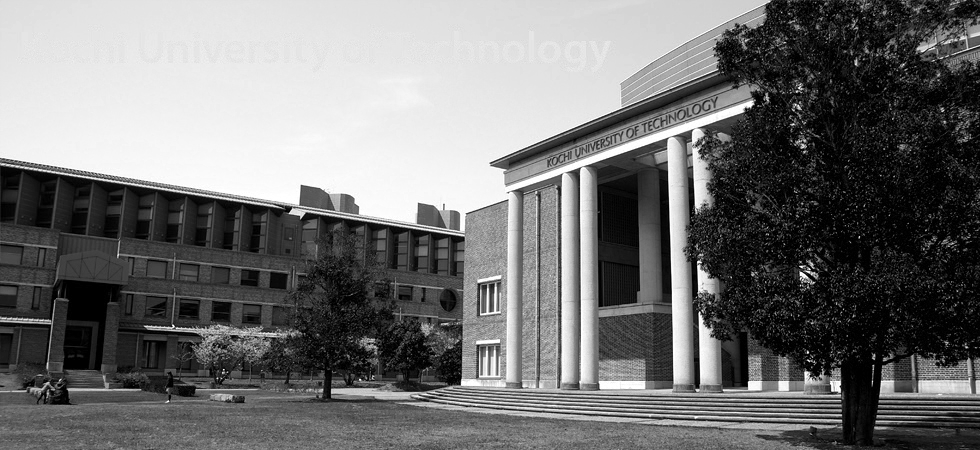
\includegraphics[keepaspectratio,width=\textwidth]{../../Figures/05_13_b.png}
        \subcaption{青チャネル}
    \end{minipage}
    \begin{minipage}[b]{.19\textwidth}
        \centering
        
\includegraphics[keepaspectratio,width=\textwidth]{../../Figures/05_14_change.png}
        \subcaption{赤青チャネル入れ替え}
    \end{minipage}
    \caption{\kadaiaa\ 実験結果}
\end{figure}
\newpage
\begin{figure}[H]
    \centering
    \begin{minipage}[b]{.23\textwidth}
        \centering
        
\includegraphics[keepaspectratio,width=\textwidth]{../../Figures/05_21_gimg.png}
        \subcaption{量子化数\ 8Bit}
        \label{fig:グレイスケール画像}
    \end{minipage}
    \begin{minipage}[b]{.23\textwidth}
        \centering
        
\includegraphics[keepaspectratio,width=\textwidth]{../../Figures/05_22_4bit.png}
        \subcaption{量子化数\ 4Bit}
    \end{minipage}
    \begin{minipage}[b]{.23\textwidth}
        \centering
        
\includegraphics[keepaspectratio,width=\textwidth]{../../Figures/05_23_2bit.png}
        \subcaption{量子化数\ 2Bit}
    \end{minipage}
    \begin{minipage}[b]{.23\textwidth}
        \centering
        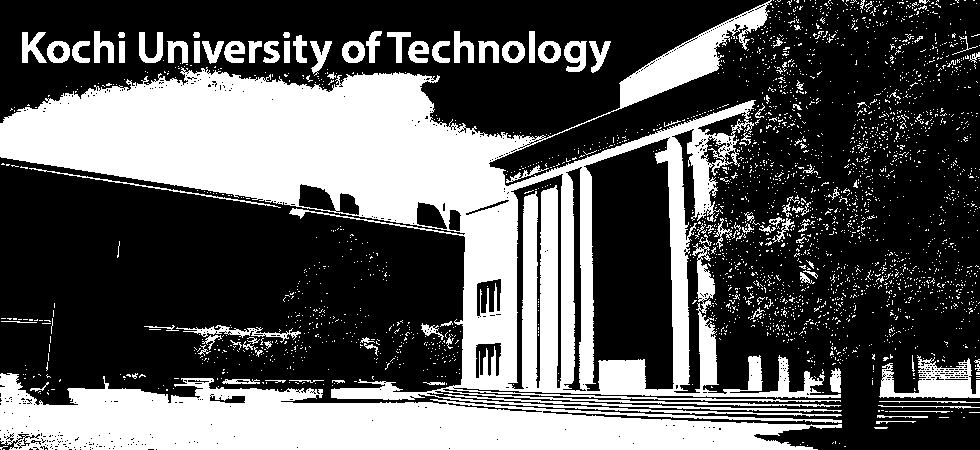
\includegraphics[keepaspectratio,width=\textwidth]{../../Figures/05_24_1bit.png}
        \subcaption{量子化数\ 1Bit}
    \end{minipage}
    \caption{\kadaiab\ 実験結果}
\end{figure}
\begin{figure}[H]
    \centering
    \begin{minipage}[b]{.23\textwidth}
        \centering
        
\includegraphics[keepaspectratio,width=\textwidth]{../../Figures/05_31_8.png}
        \subcaption{量子化数\ 8Bit}
    \end{minipage}
    \begin{minipage}[b]{.23\textwidth}
        \centering
        
\includegraphics[keepaspectratio,width=\textwidth]{../../Figures/05_32_4.png}
        \subcaption{量子化数\ 4Bit}
    \end{minipage}
    \begin{minipage}[b]{.23\textwidth}
        \centering
        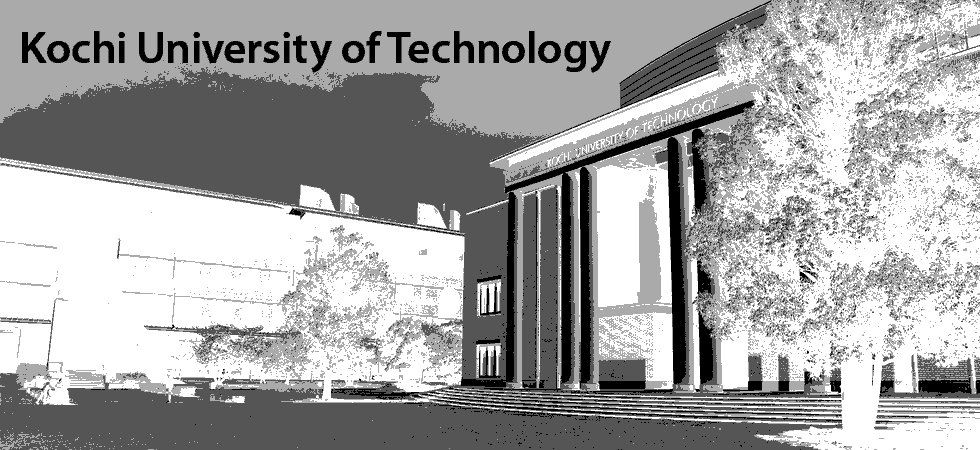
\includegraphics[keepaspectratio,width=\textwidth]{../../Figures/05_33_2.png}
        \subcaption{量子化数\ 2Bit}
    \end{minipage}
    \begin{minipage}[b]{.23\textwidth}
        \centering
        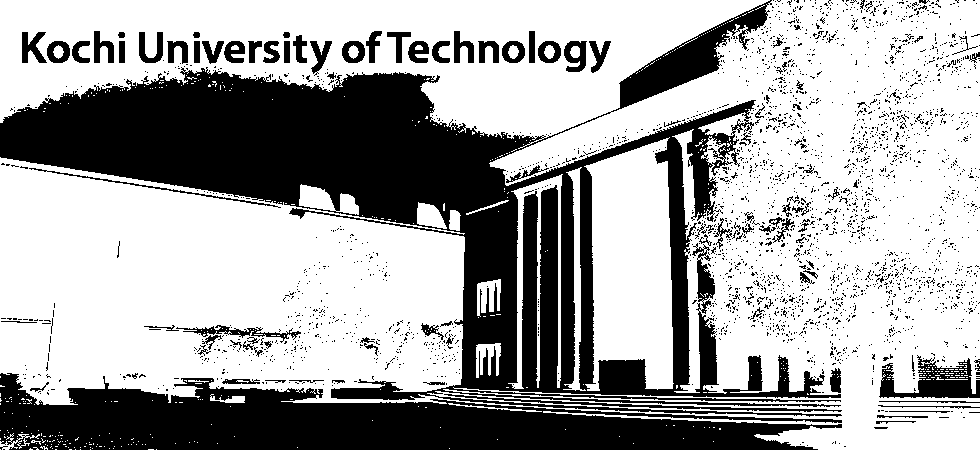
\includegraphics[keepaspectratio,width=\textwidth]{../../Figures/05_34_1.png}
        \subcaption{量子化数\ 1Bit}
    \end{minipage}
    \caption{\kadaiac\ 実験結果}
\end{figure}
\begin{figure}[H]
    \centering
    \begin{minipage}[b]{.7\textwidth}
        \centering
        \begin{minipage}[b]{.3\textwidth}
            \centering
            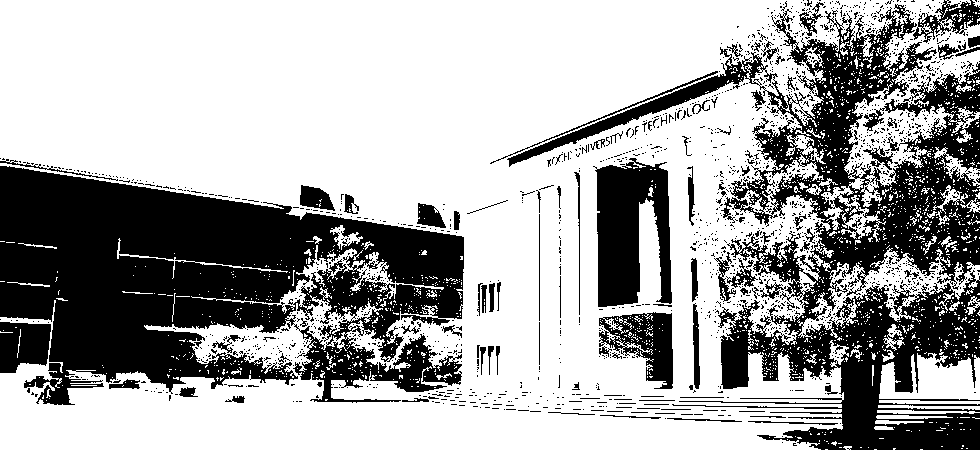
\includegraphics[keepaspectratio,width=\textwidth]{../../Figures/05_41.png}
            \subcaption{閾値\ \(64\)}
        \end{minipage}
        \begin{minipage}[b]{.3\textwidth}
            \centering
            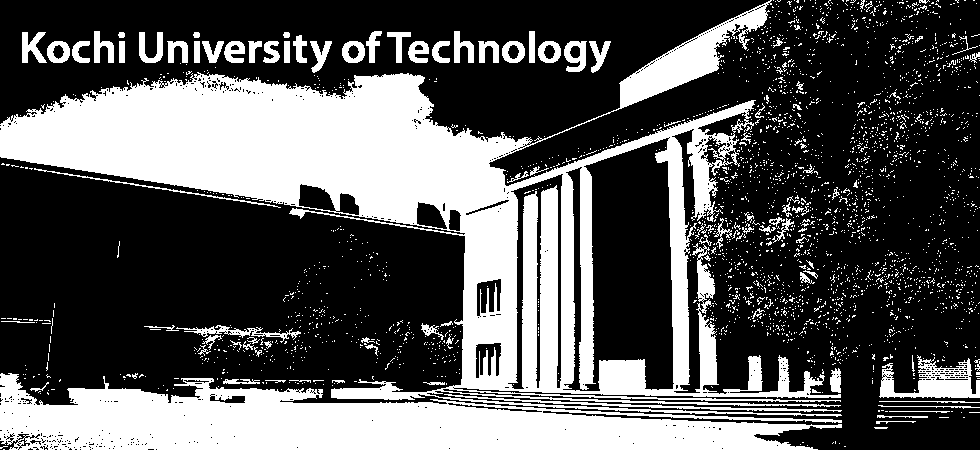
\includegraphics[keepaspectratio,width=\textwidth]{../../Figures/05_42.png}
            \subcaption{閾値\ \(128\)}
        \end{minipage}
        \begin{minipage}[b]{.3\textwidth}
            \centering
            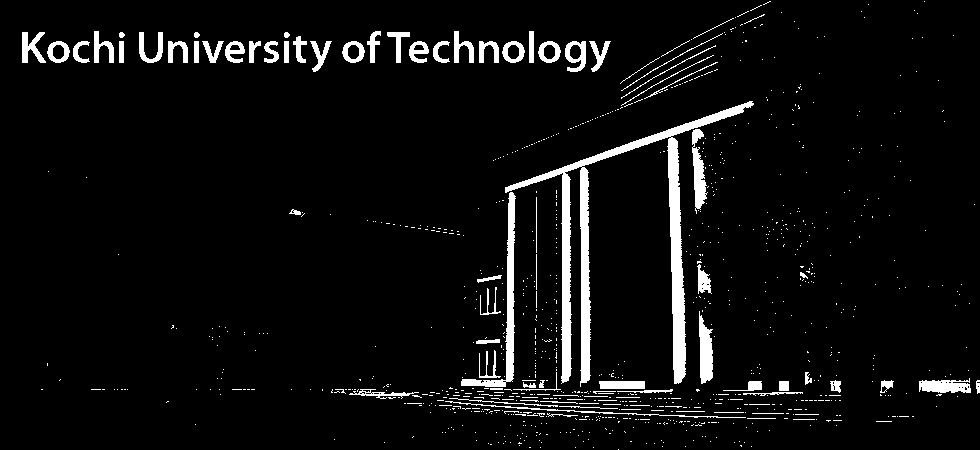
\includegraphics[keepaspectratio,width=\textwidth]{../../Figures/05_43.png}
            \subcaption{閾値\ \(192\)}
        \end{minipage}
        \caption{\kadaiad\ 実験結果}
    \end{minipage}
    \begin{minipage}[b]{.25\textwidth}
        \centering
        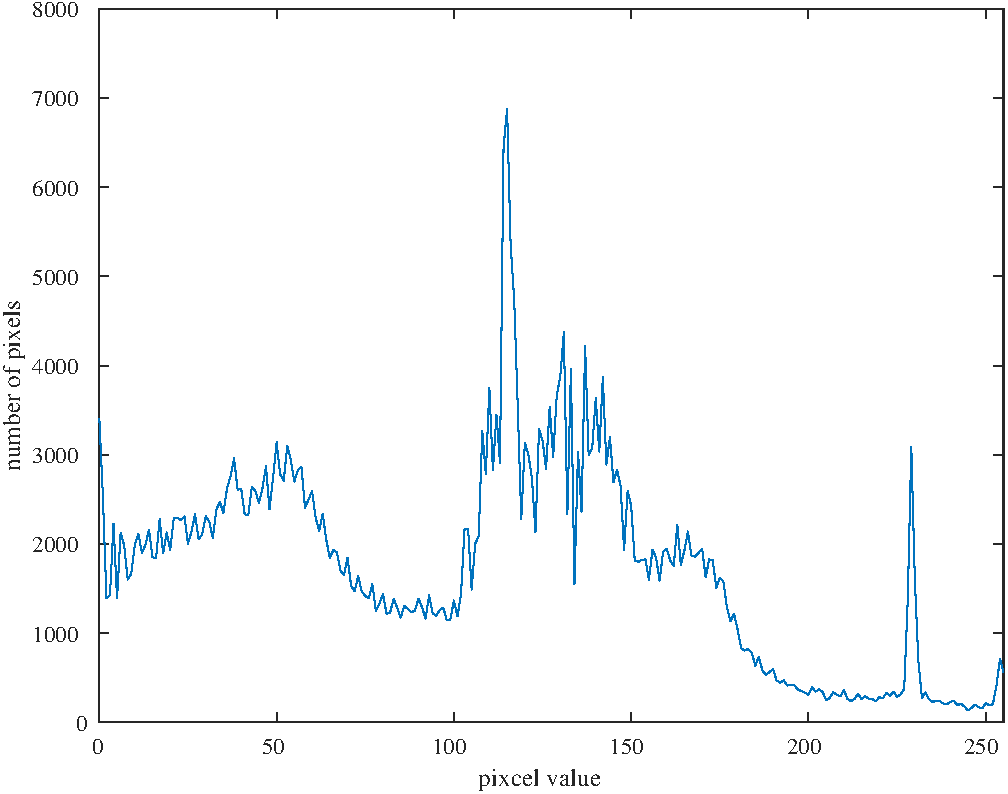
\includegraphics[keepaspectratio,width=\textwidth]{../../Figures/05_50_graph.pdf}
        \caption{画素値ヒストグラム\footnotemark[1]}
    \end{minipage}
\end{figure}
\begin{figure}[H]
    \centering
    \begin{minipage}[b]{.49\textwidth}
        \centering
        \begin{minipage}[b]{.3\textwidth}
            \centering
            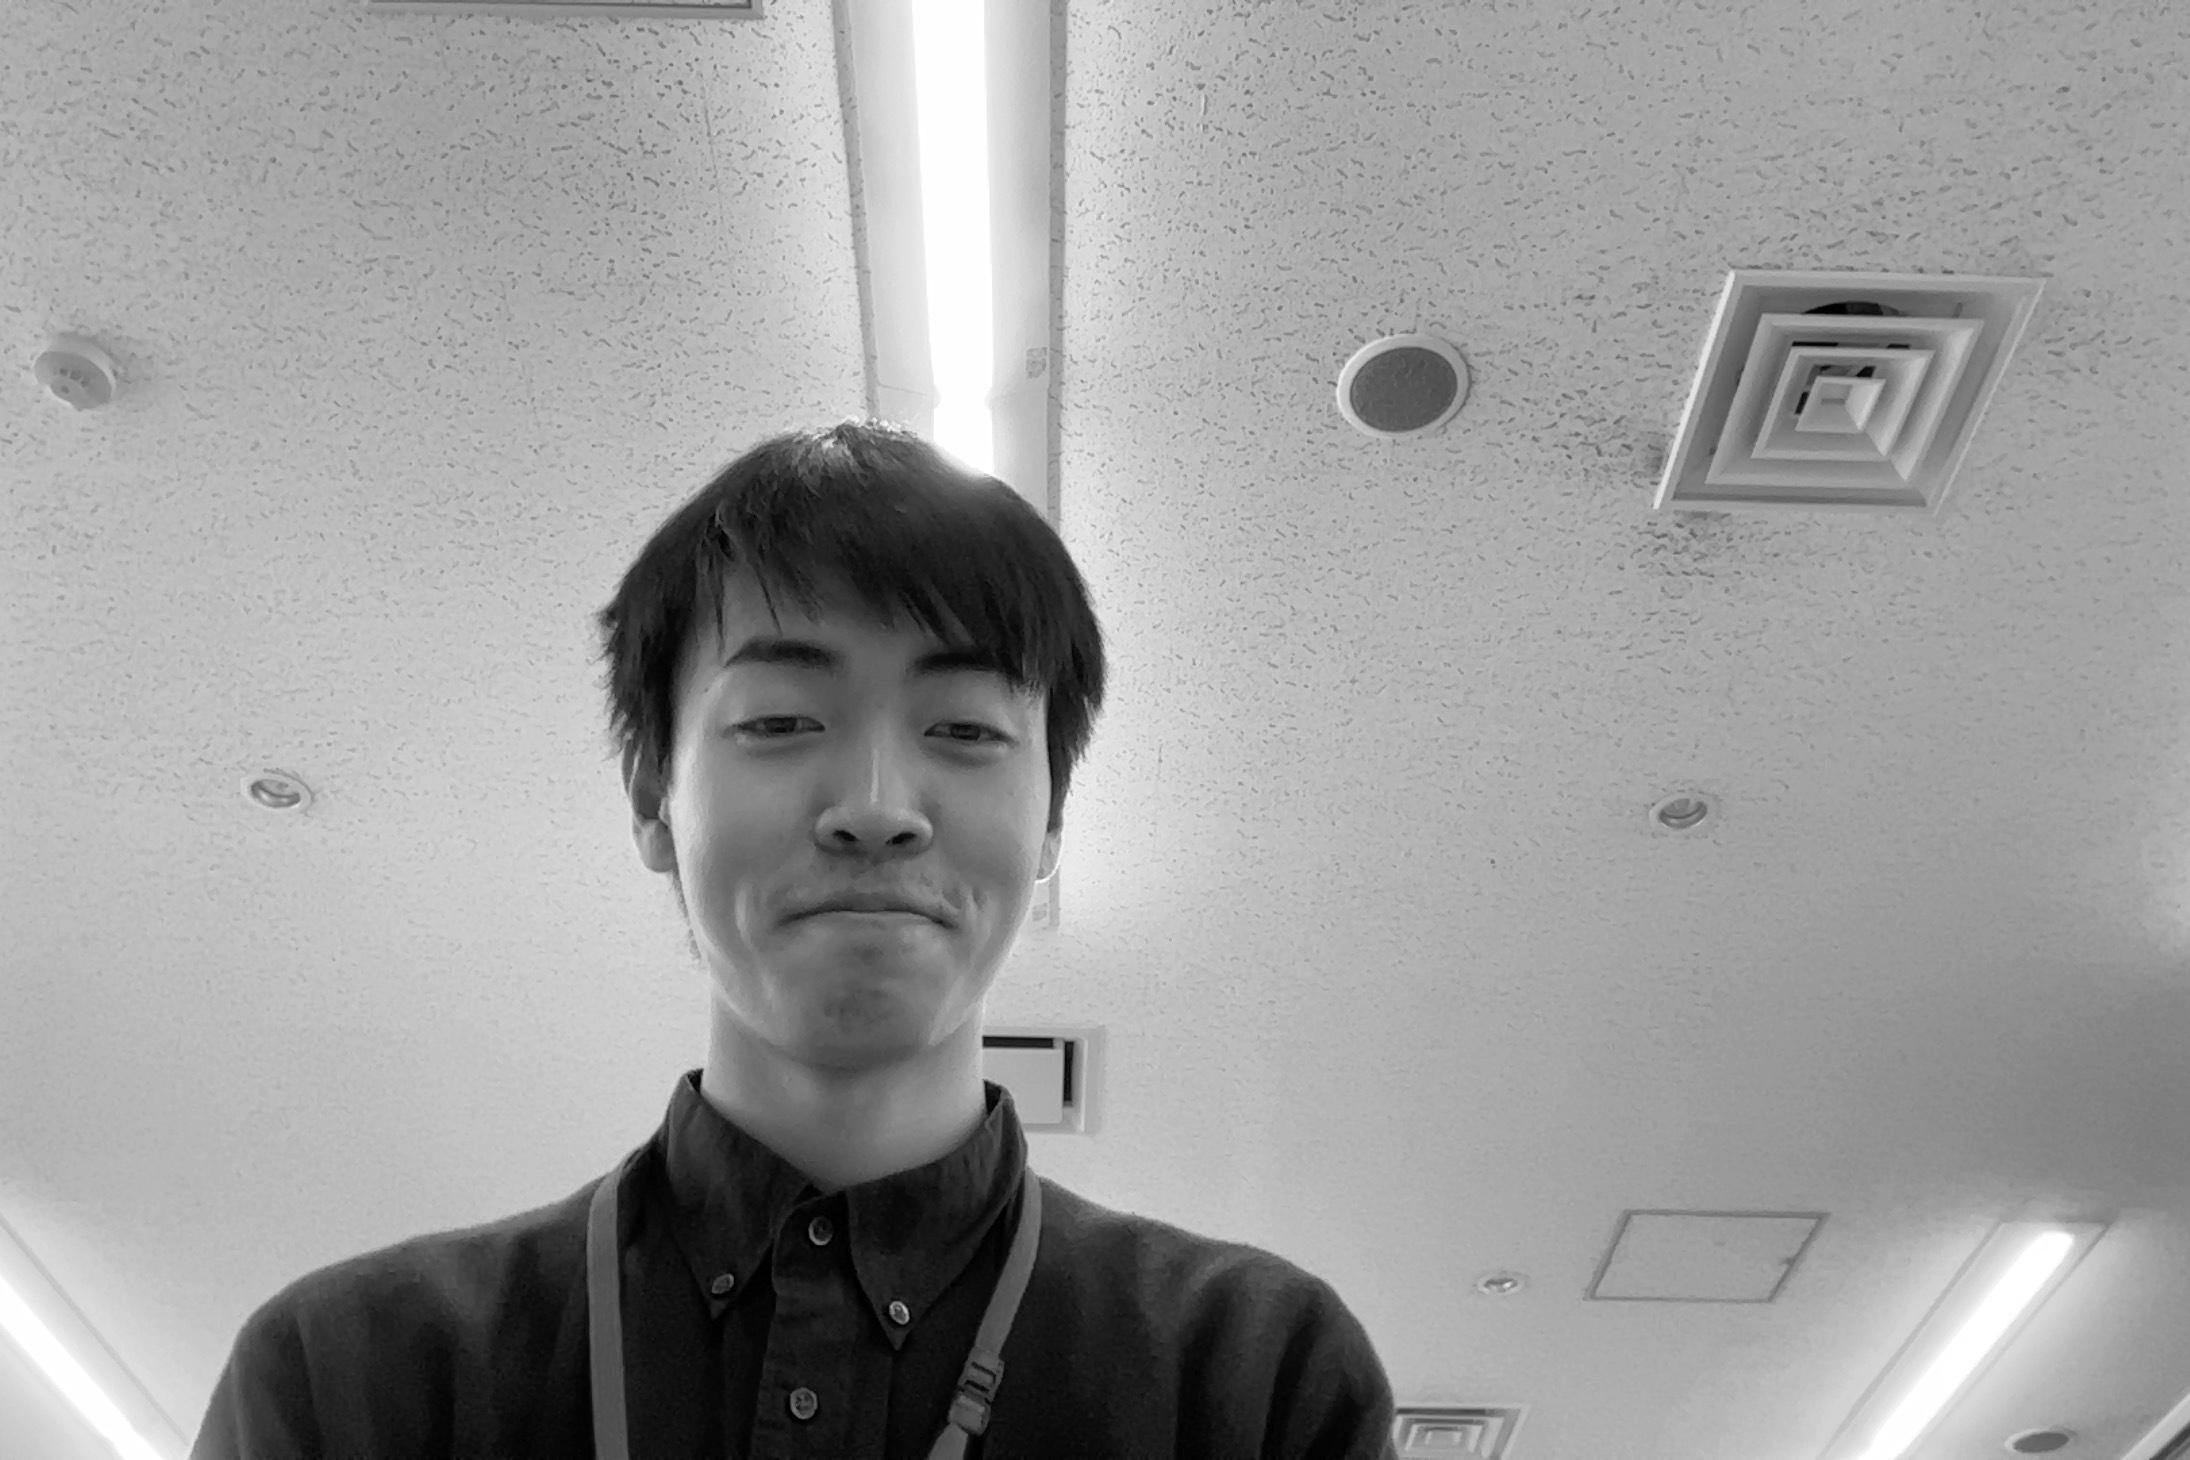
\includegraphics[keepaspectratio,width=\textwidth]{../../05_UnderstandingImages/fig1_g.jpg}
            \subcaption{被写体と背景}
        \end{minipage}
        \begin{minipage}[b]{.3\textwidth}
            \centering
            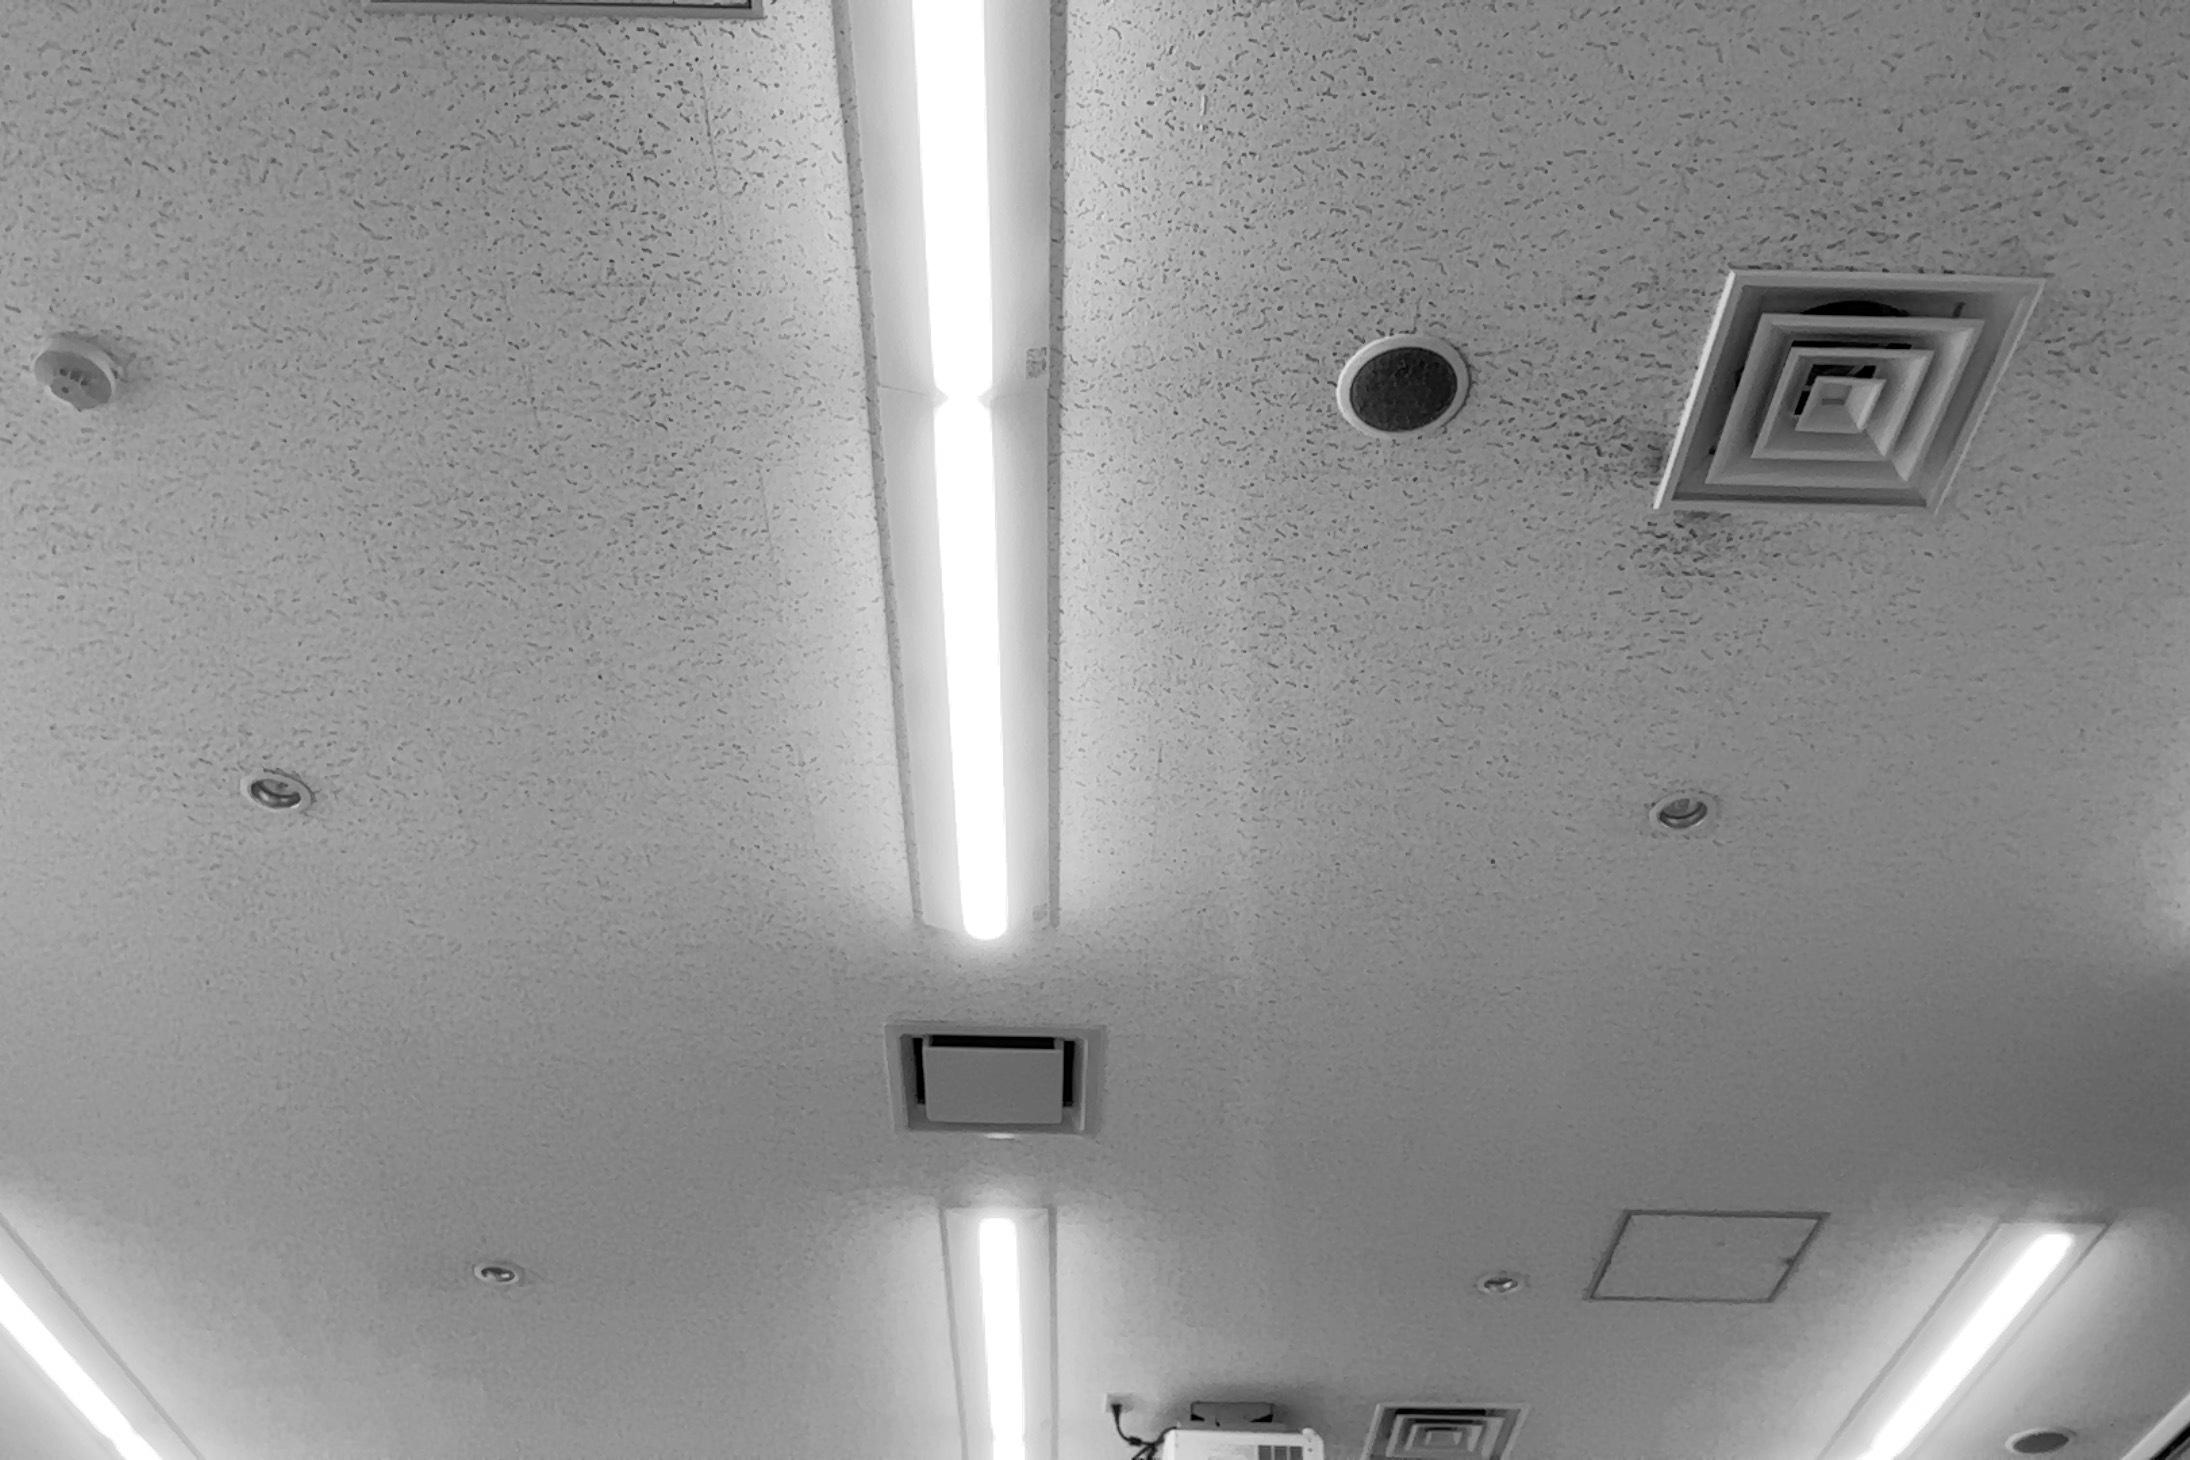
\includegraphics[keepaspectratio,width=\textwidth]{../../05_UnderstandingImages/fig2_g.jpg}
            \subcaption{背景のみ}
        \end{minipage}
        \begin{minipage}[b]{.3\textwidth}
            \centering
            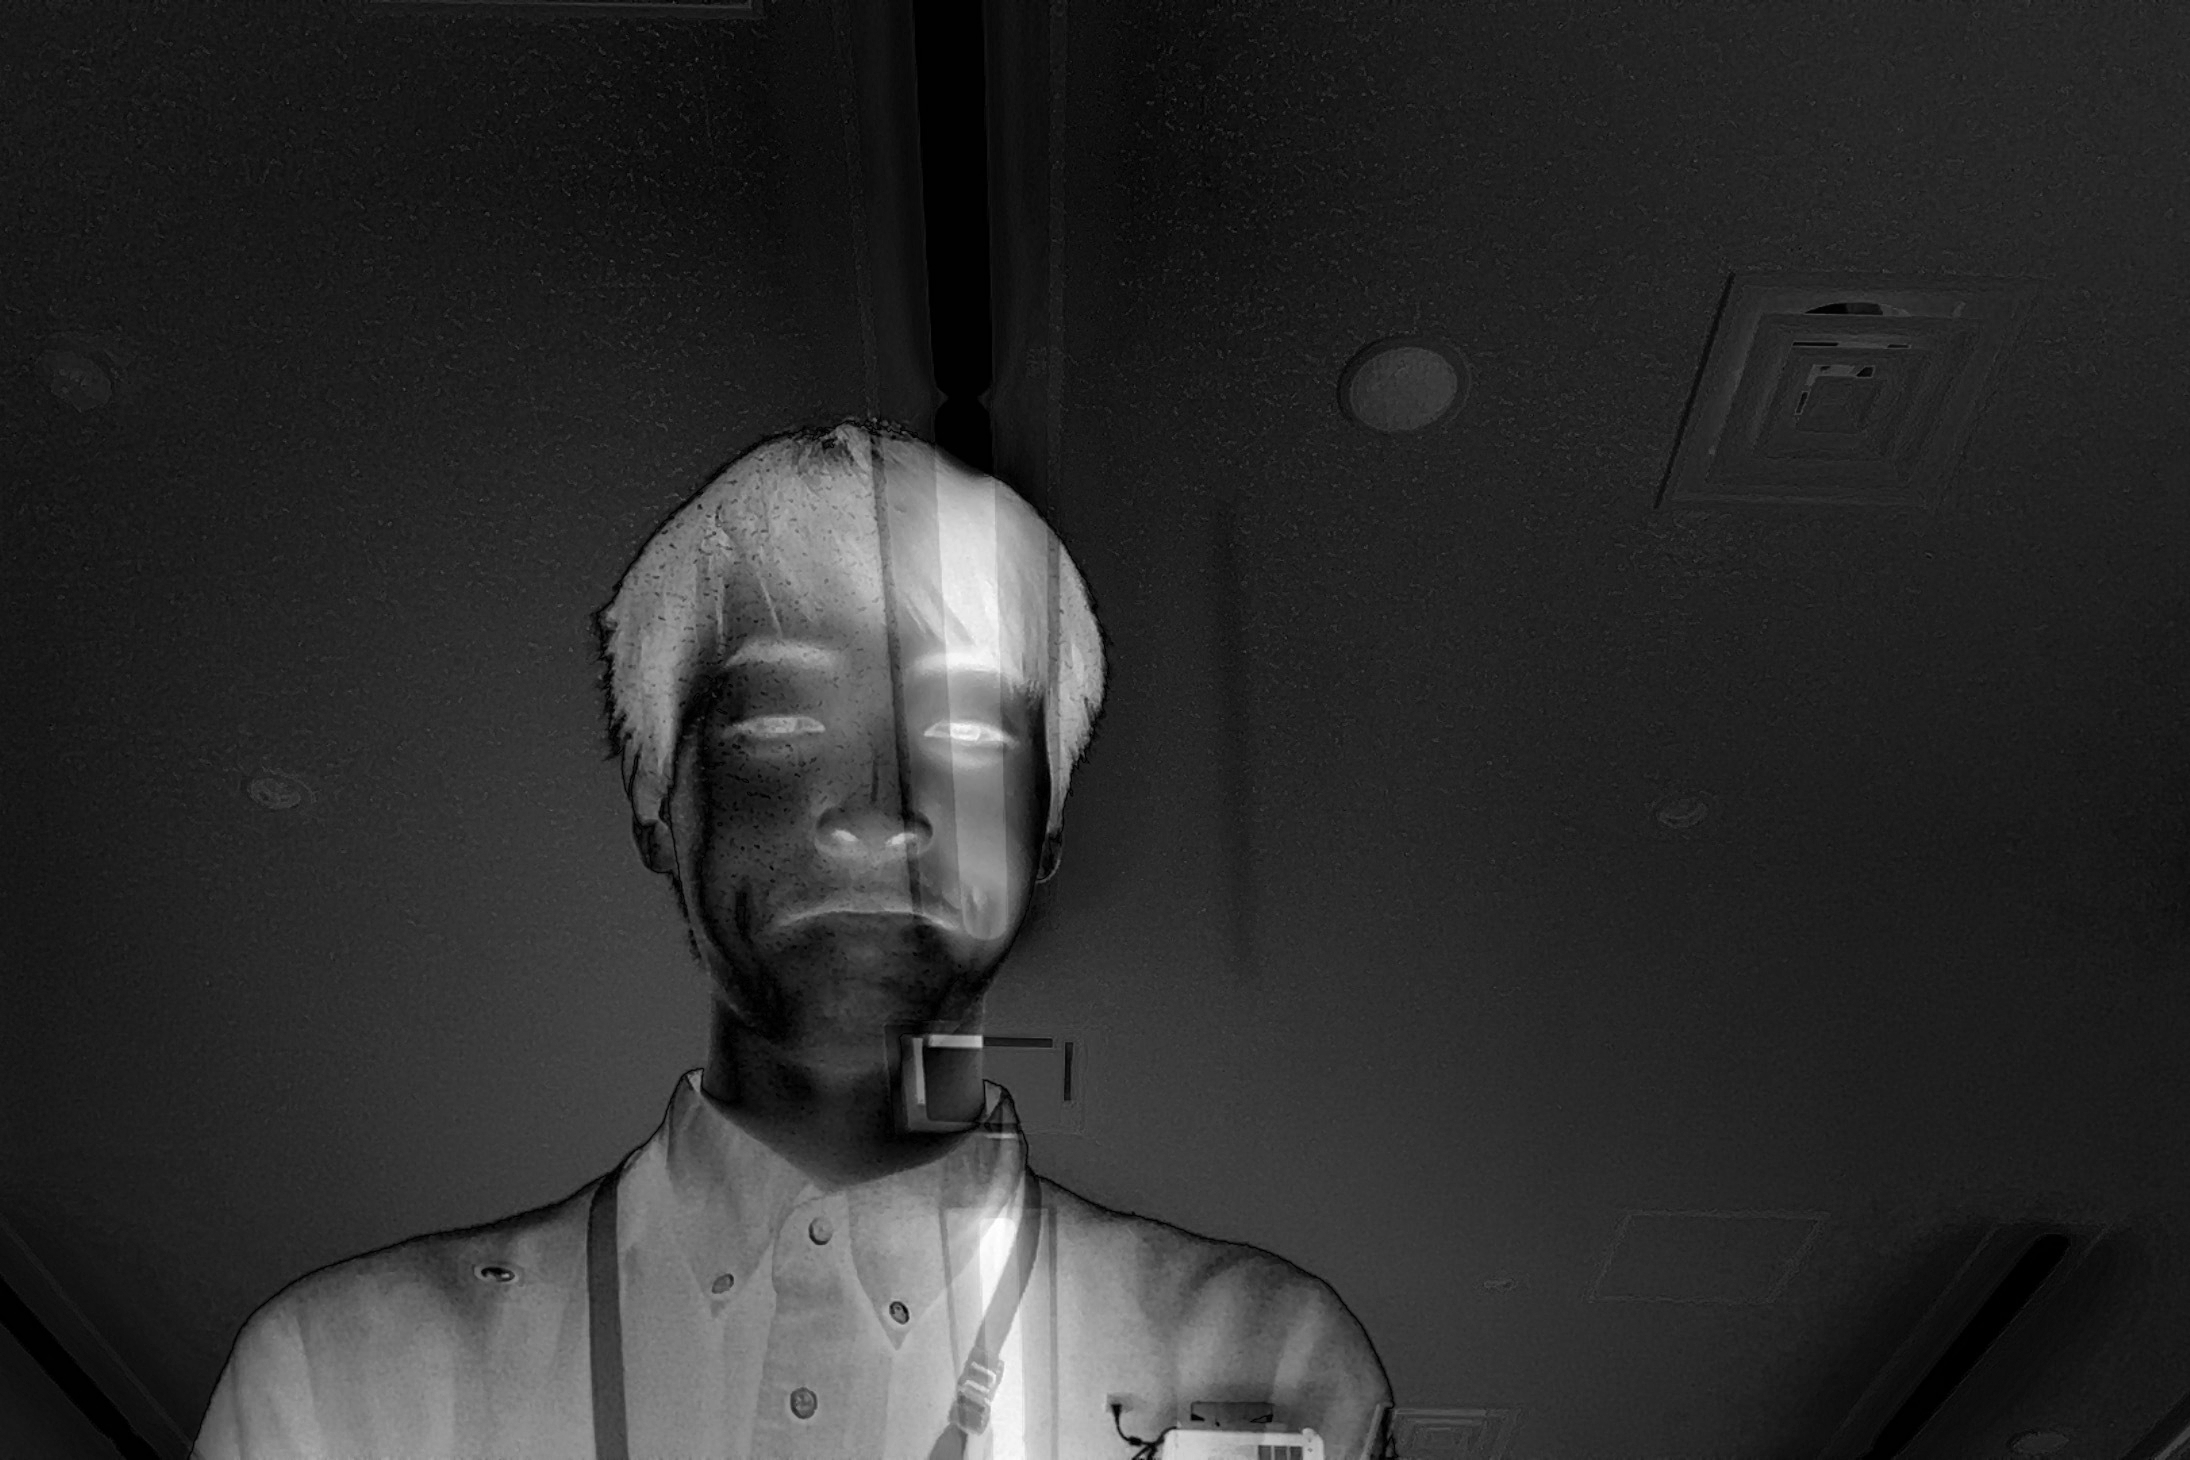
\includegraphics[keepaspectratio,width=\textwidth]{../../Figures/05_60.png}
            \subcaption{背景差分画像}
        \end{minipage}
        \caption{\kadaiaf\ 実験結果}
    \end{minipage}
    \nextfloat
    \begin{minipage}[b]{.49\textwidth}
        \centering
        \begin{minipage}[b]{.3\textwidth}
            \centering
            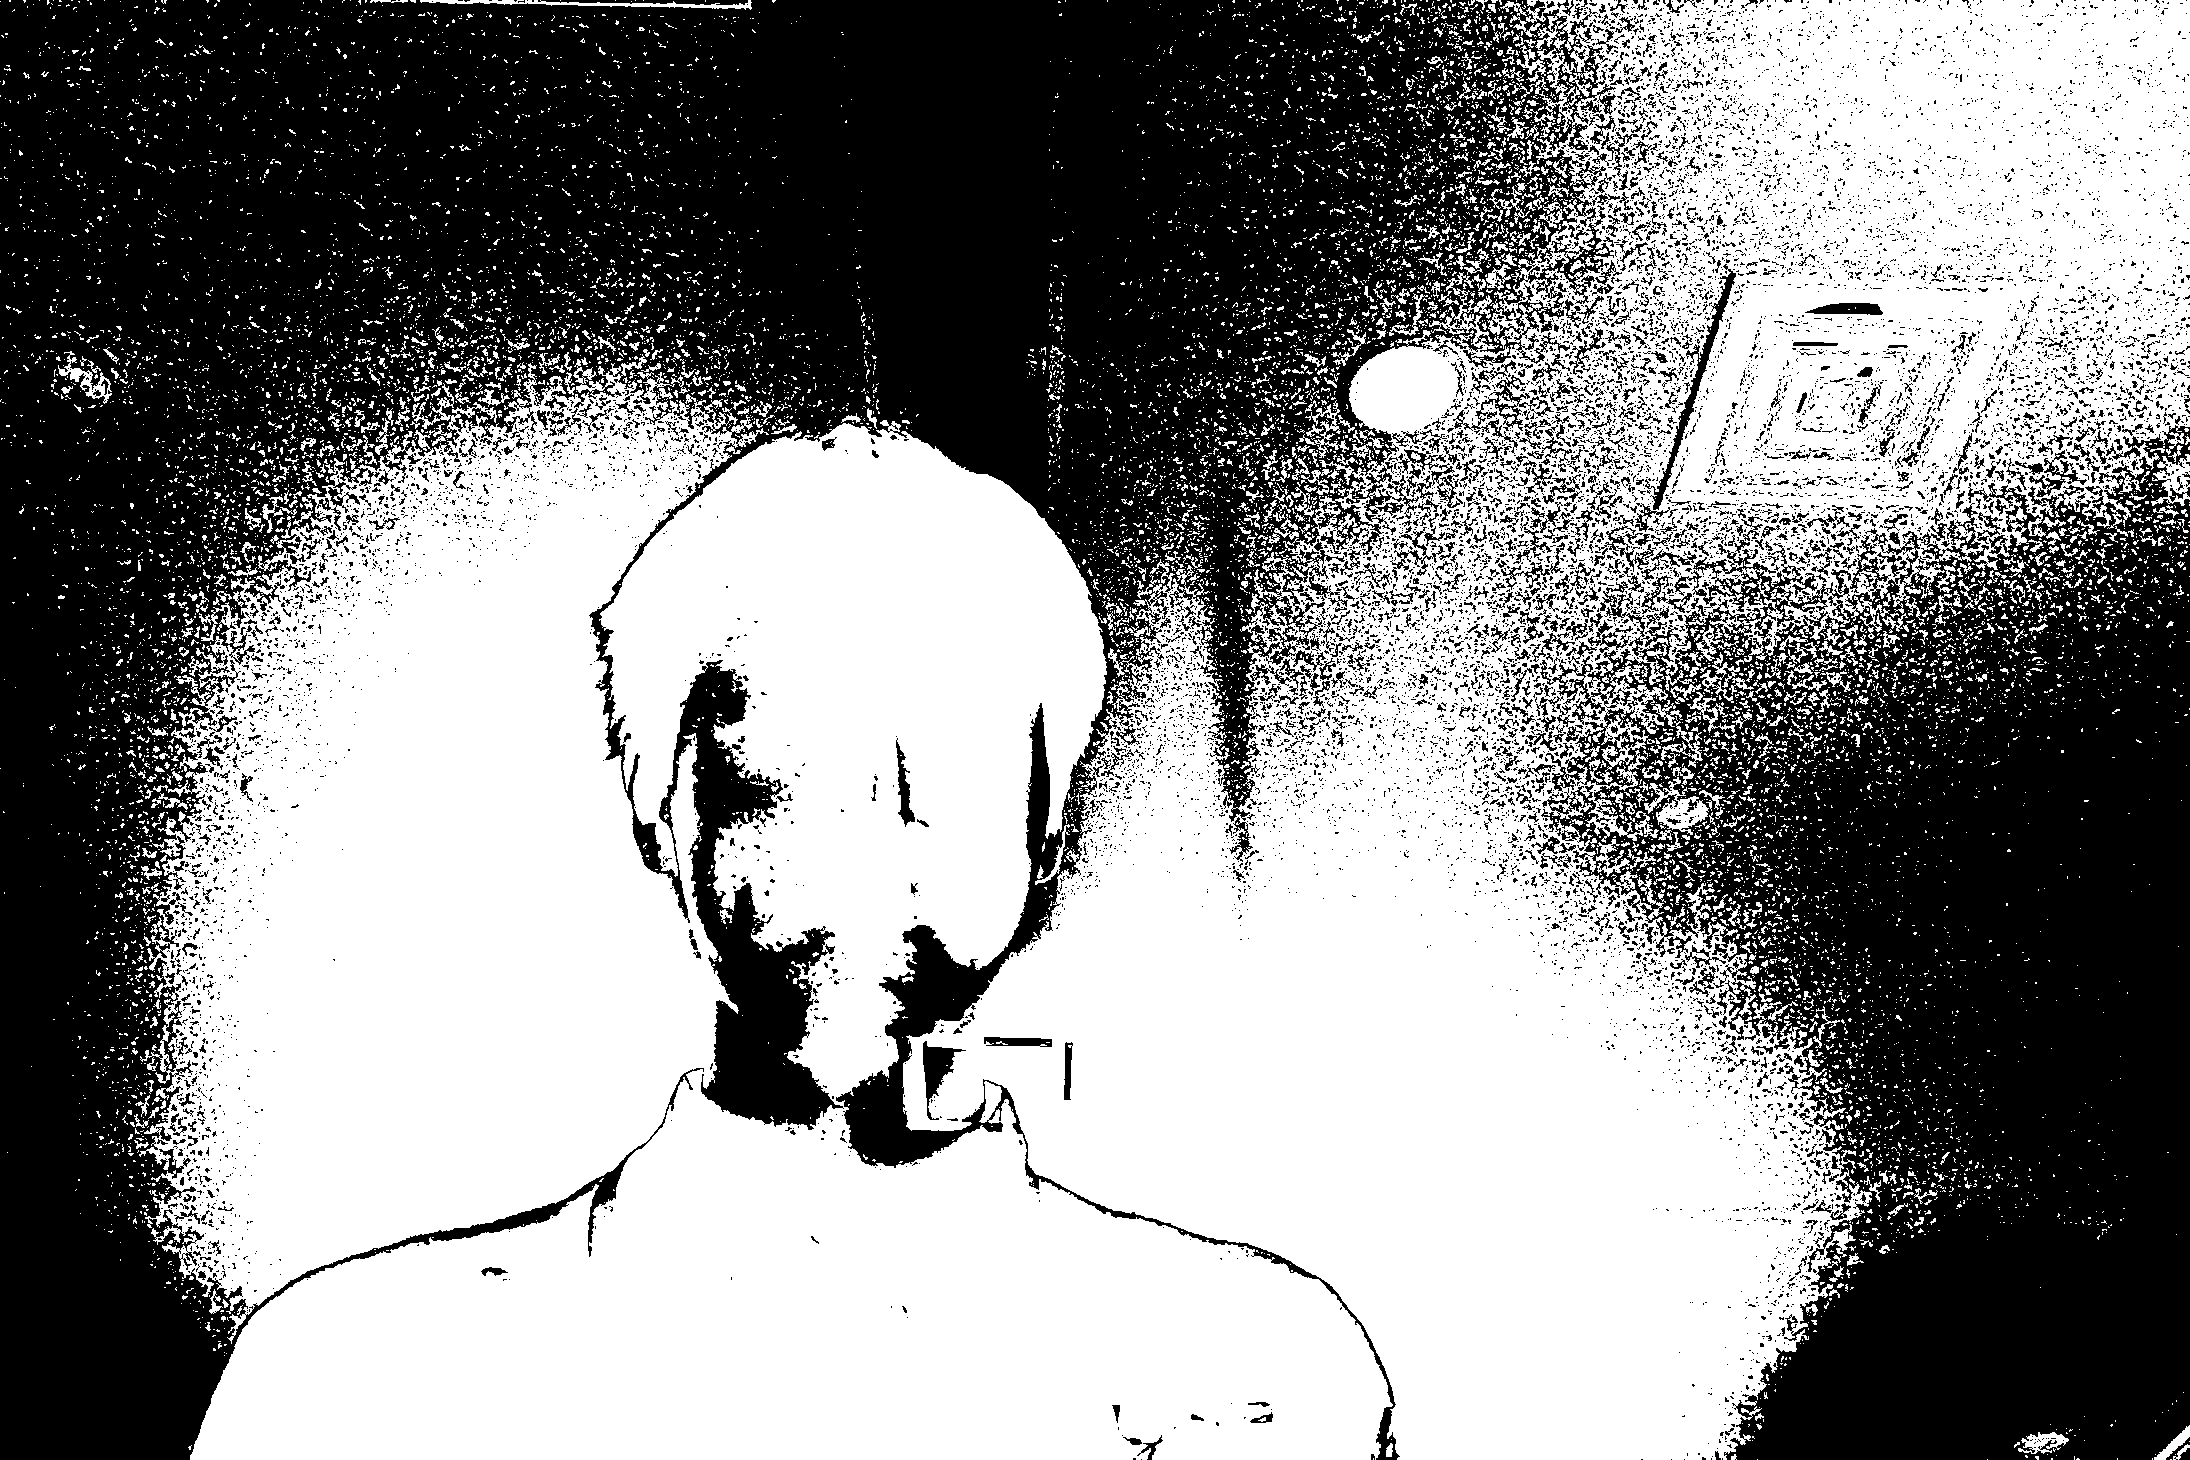
\includegraphics[keepaspectratio,width=\textwidth]{../../Figures/05_61.png}
            \subcaption{閾値\ \(32\)}
        \end{minipage}
        \begin{minipage}[b]{.3\textwidth}
            \centering
            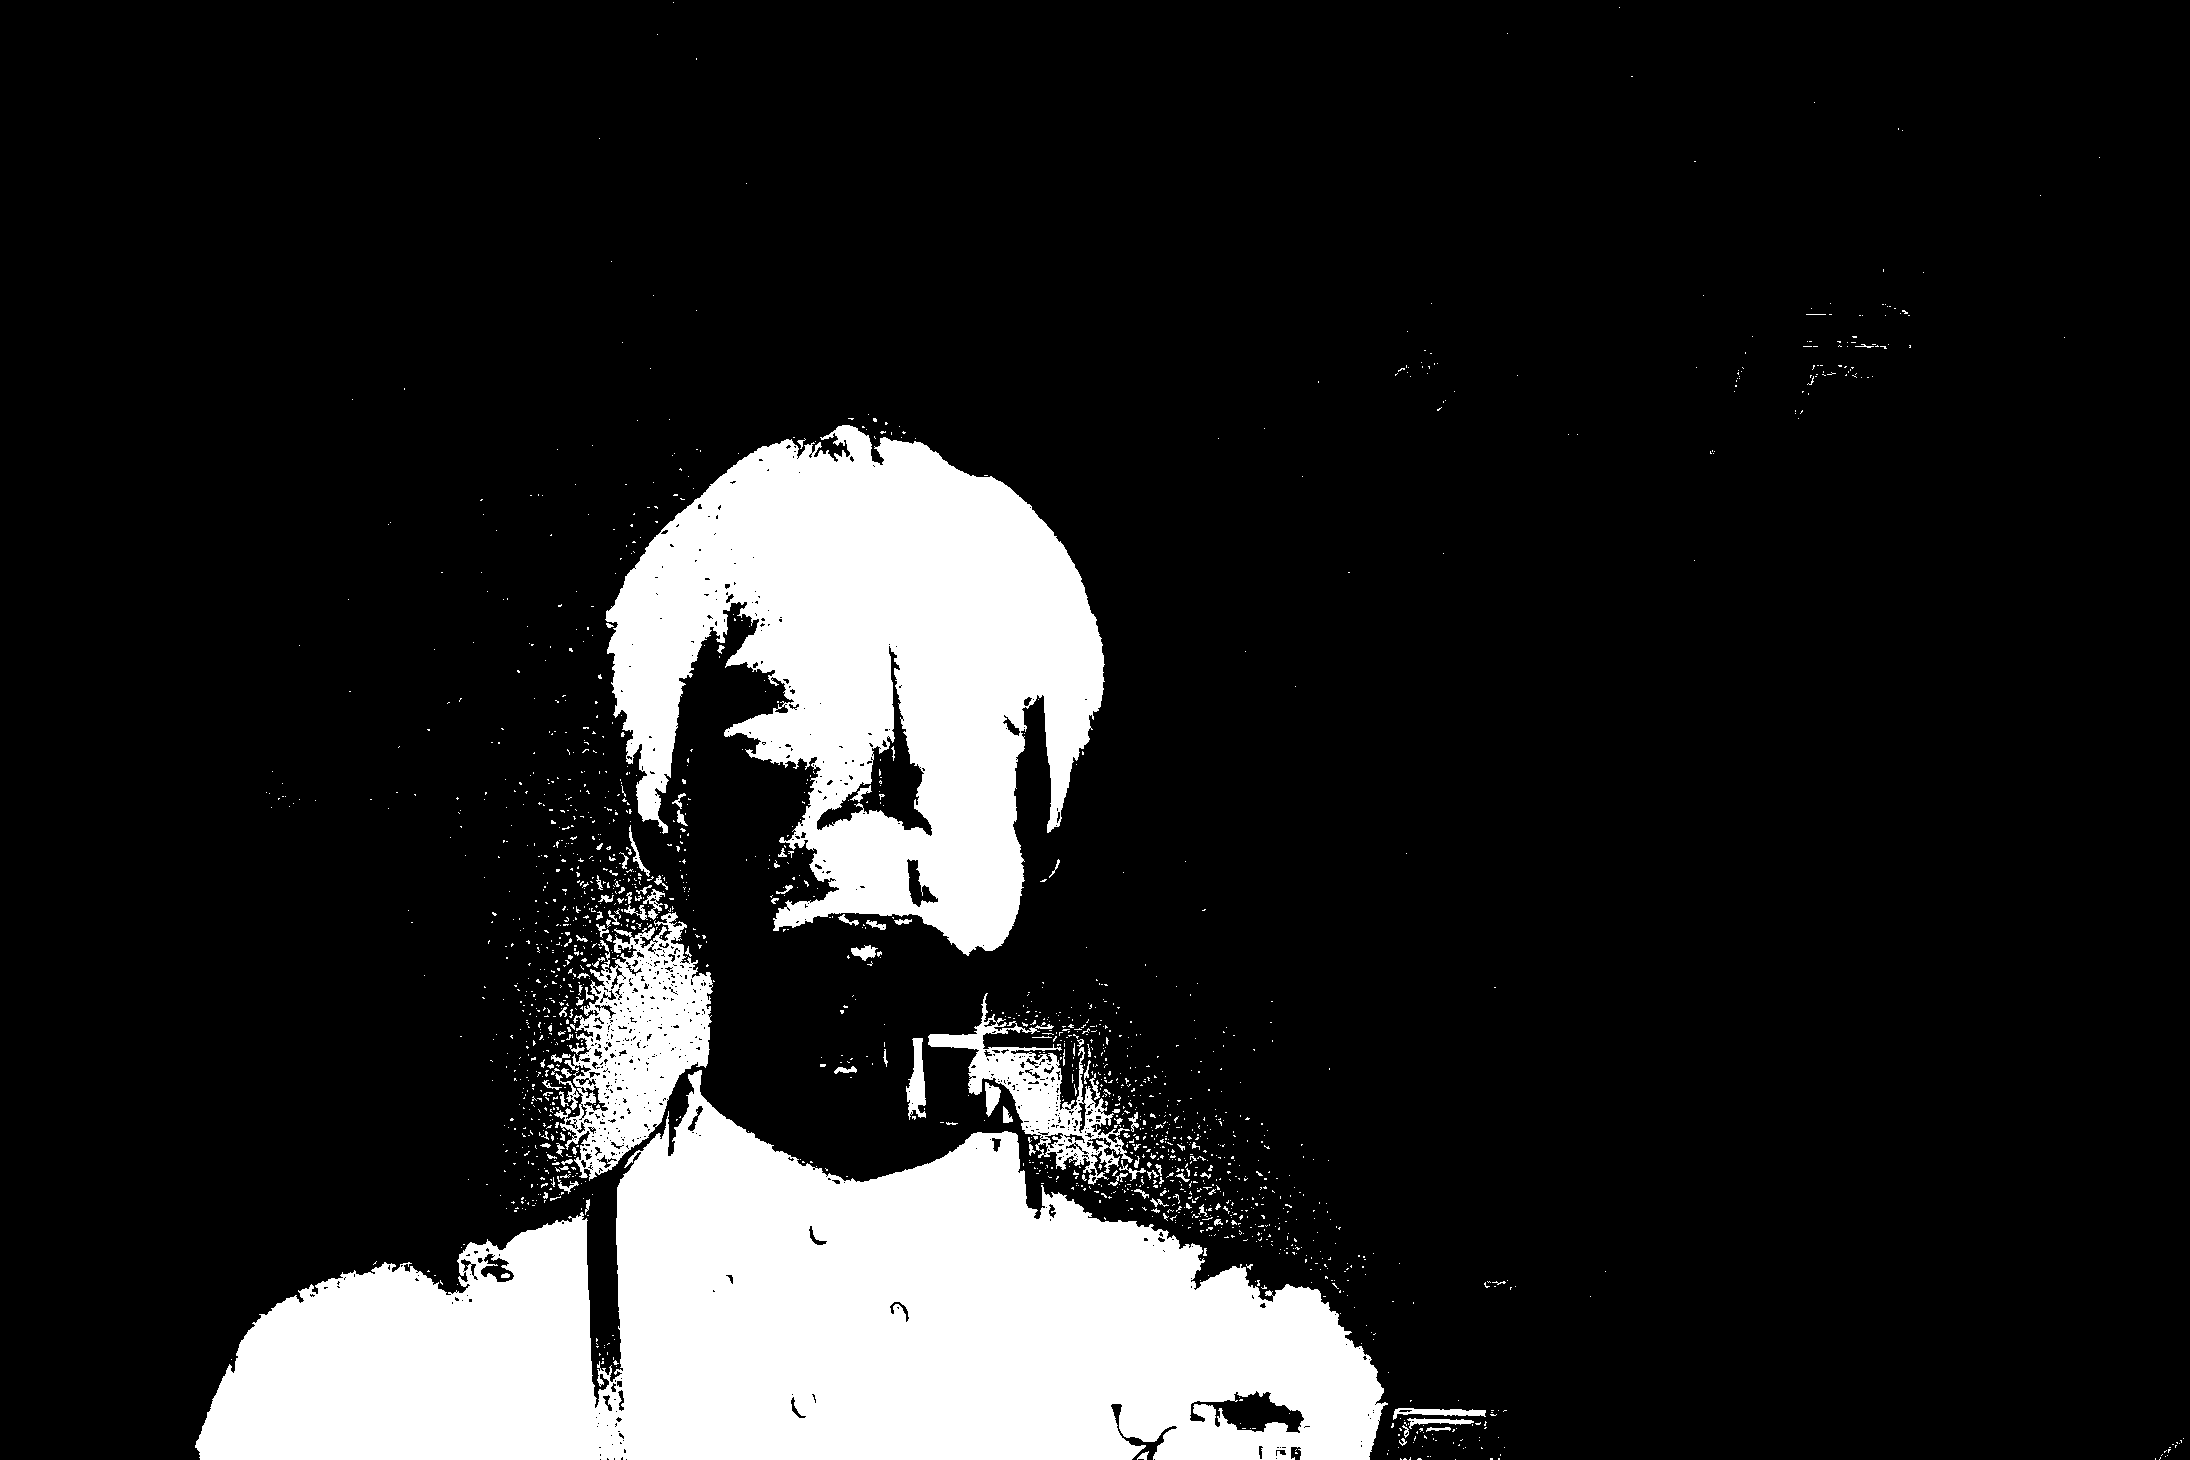
\includegraphics[keepaspectratio,width=\textwidth]{../../Figures/05_62.png}
            \subcaption{閾値\ \(64\)}
        \end{minipage}
        \begin{minipage}[b]{.3\textwidth}
            \centering
            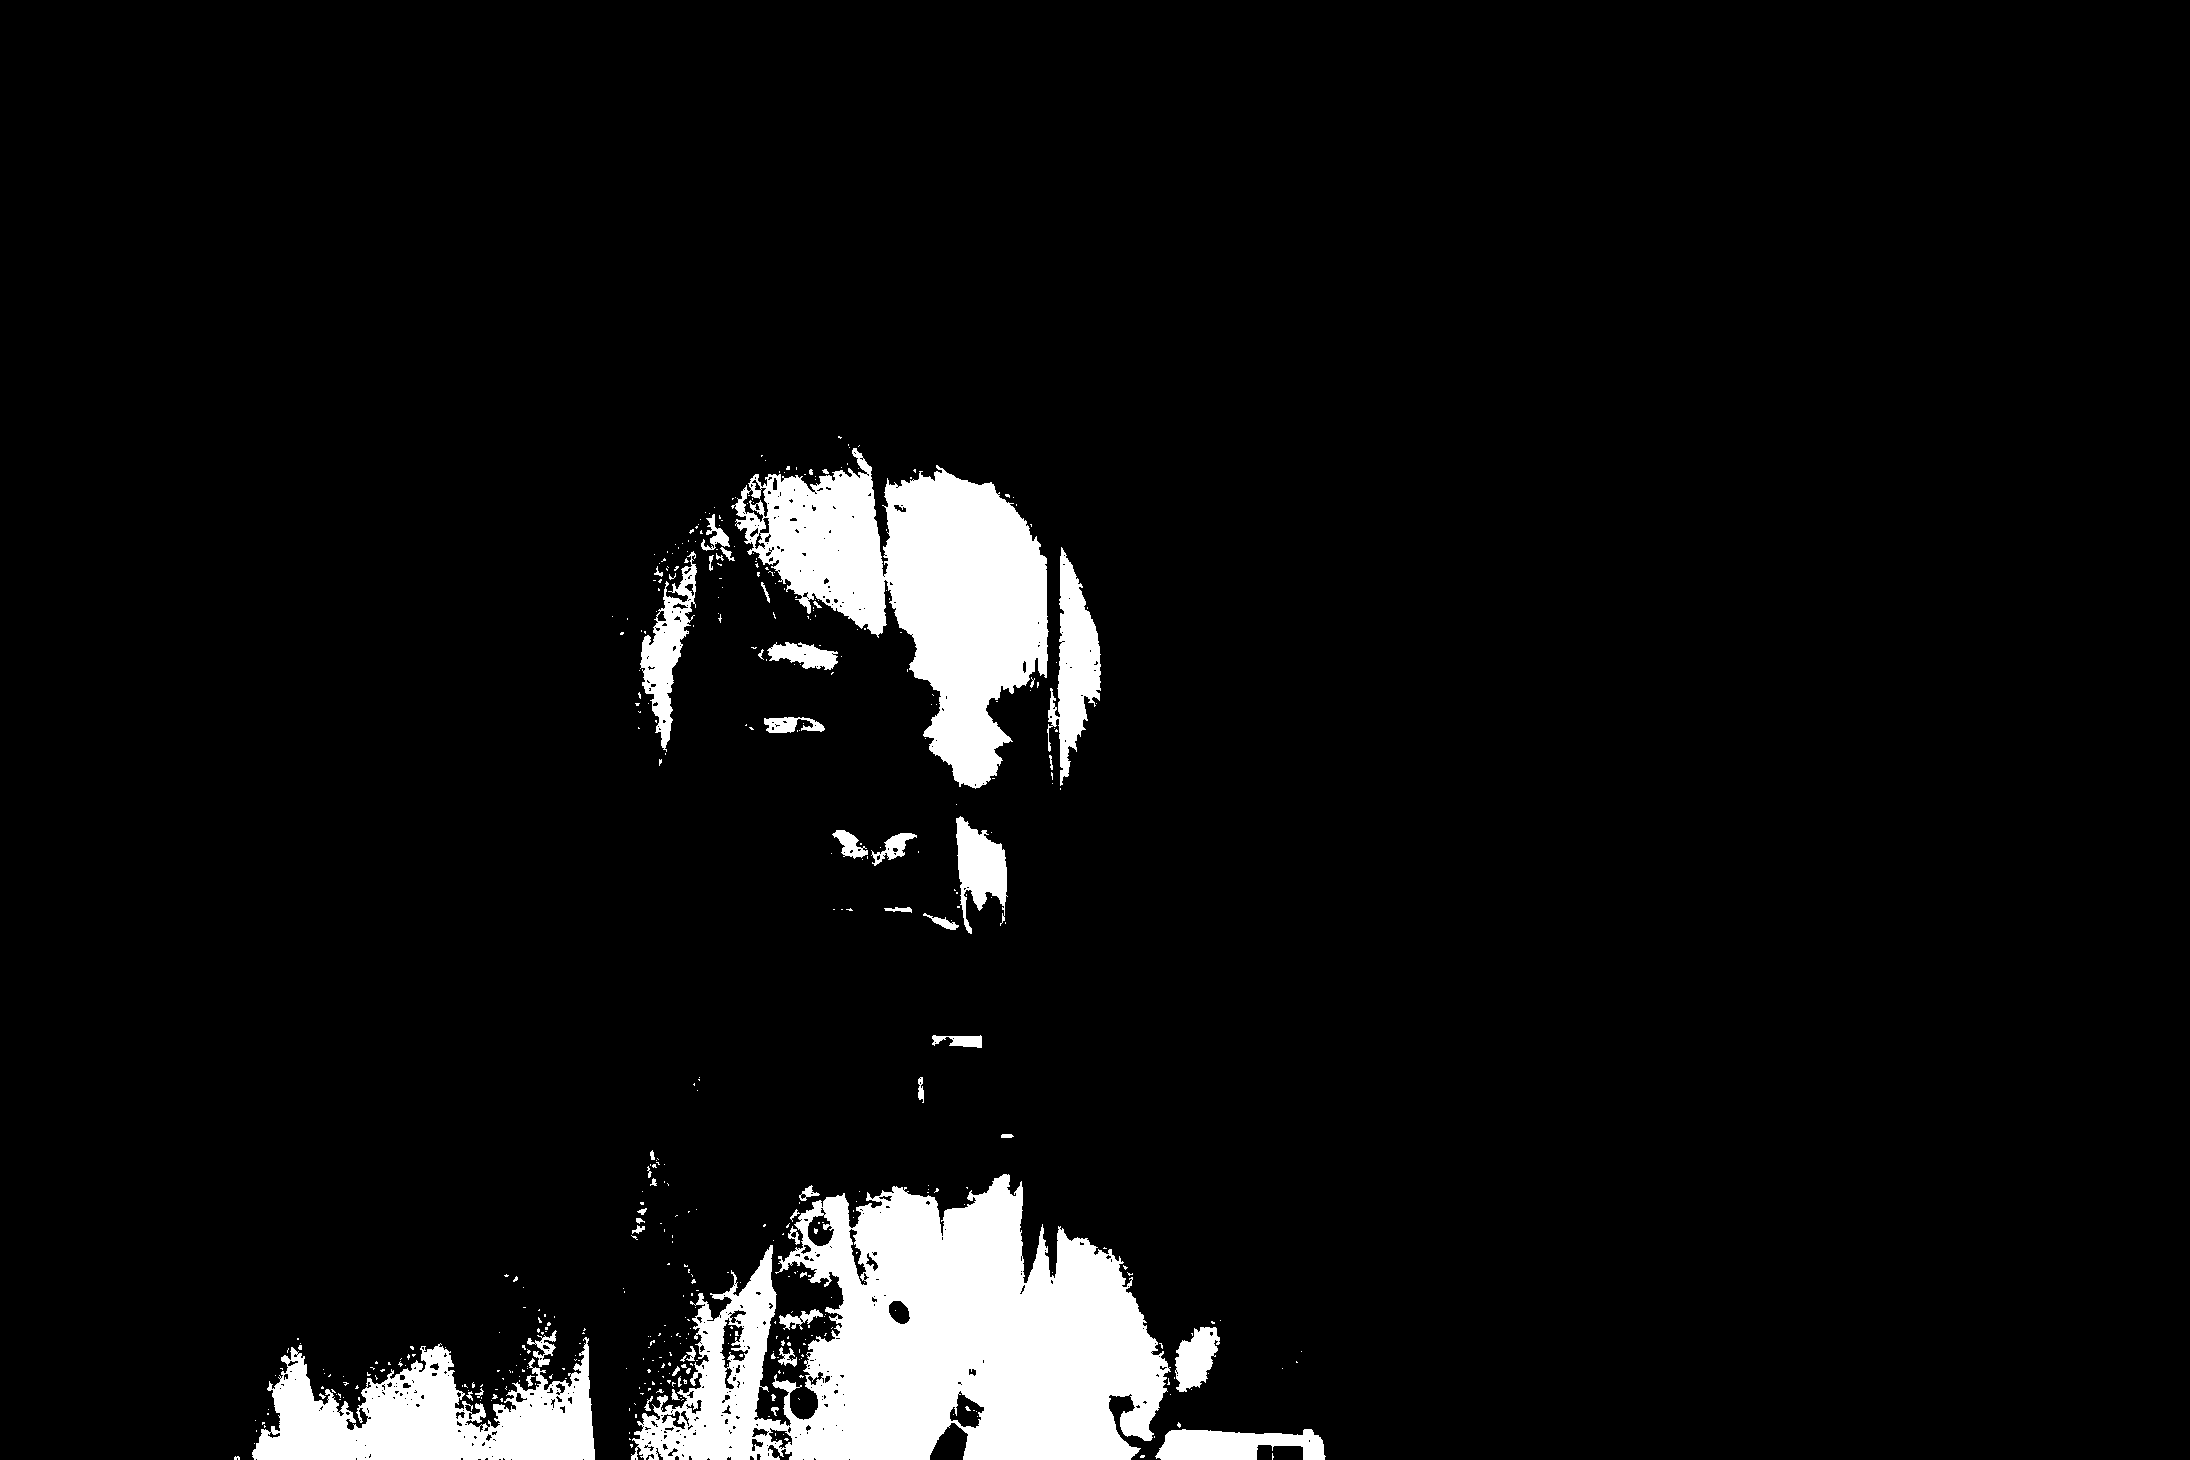
\includegraphics[keepaspectratio,width=\textwidth]{../../Figures/05_63.png}
            \subcaption{閾値\ \(128\)}
        \end{minipage}
        \caption{背景差分画像の閾値処理}
    \end{minipage}
\end{figure}
\footnotetext[1]{\figref{fig:グレイスケール画像}の画素値ヒストグラム}
\begin{figure}[h]
    \centering
    \begin{minipage}[b]{.3\textwidth}
        \centering
        
\includegraphics[keepaspectratio,width=\textwidth]{../../Figures/05_21_gimg.png}
        \subcaption{元画像}
    \end{minipage}
    \begin{minipage}[b]{.3\textwidth}
        \centering
        
\includegraphics[keepaspectratio,width=\textwidth]{../../06_ImageFiltering/file_white-Gaussian-Noise.png}
        \subcaption{白色ガウス雑音画像(\wgnimg)}
    \end{minipage}
    \begin{minipage}[b]{.3\textwidth}
        \centering
        
\includegraphics[keepaspectratio,width=\textwidth]{../../06_ImageFiltering/file_impluse-noise.png}
        \subcaption{インパルス雑音画像(\inimg)}
    \end{minipage}
    \caption{\kadaiaa\ 実験結果}
\end{figure}
\paragraph{平滑化フィルタ,メディアンフィルタ}
\wgnimg に対して平滑化フィルタを適用すると,雑音部分が目立たなくなった.また,\inimg に対して平滑化フィルタを適用すると,雑音が取り除かれることなく残った.
\wgnimg と\inimg に対してメディアンフィルタを適用すると,雑音部分が目立たなくなった.
\begin{figure}[H]
    \centering
    \begin{minipage}[b]{.49\textwidth}
        \begin{minipage}[b]{.49\textwidth}
            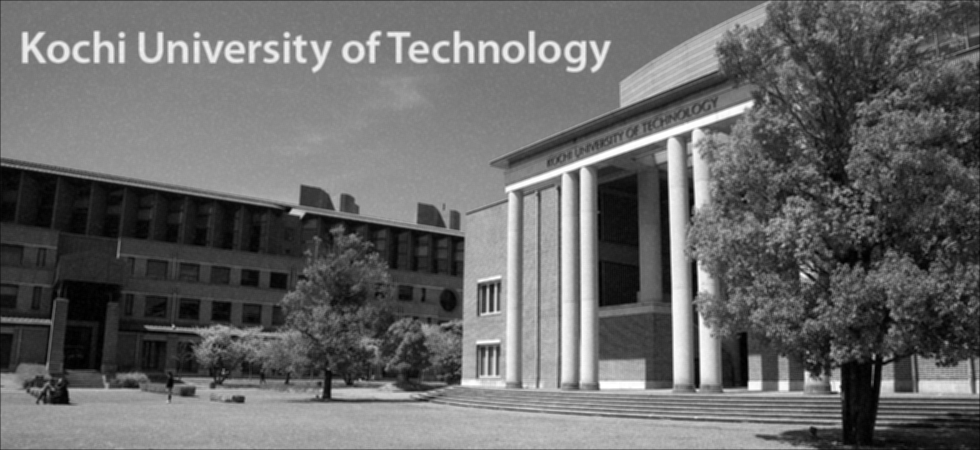
\includegraphics[keepaspectratio,width=\textwidth]{../../Figures/06_21_sf_img_wgn.png}
            \subcaption{\wgnimg}
        \end{minipage}
        \begin{minipage}[b]{.49\textwidth}
            
\includegraphics[keepaspectratio,width=\textwidth]{../../Figures/06_22_sf_img_in.png}
            \subcaption{\inimg}
        \end{minipage}
        \caption{平滑化フィルタ適用後の画像}
    \end{minipage}
    \begin{minipage}[b]{.49\textwidth}
        \begin{minipage}[b]{.49\textwidth}
            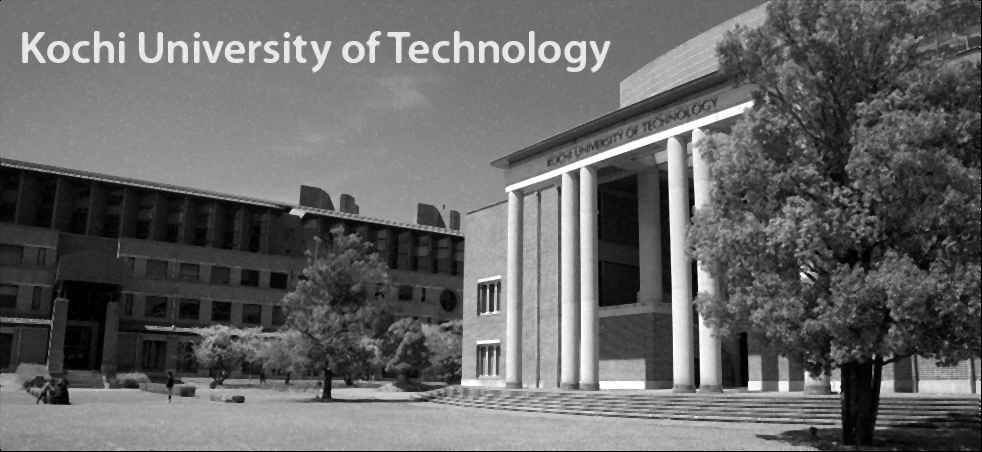
\includegraphics[keepaspectratio,width=\textwidth]{../../Figures/06_23_mf_img_wgn.png}
            \subcaption{\wgnimg}
        \end{minipage}
        \begin{minipage}[b]{.49\textwidth}
            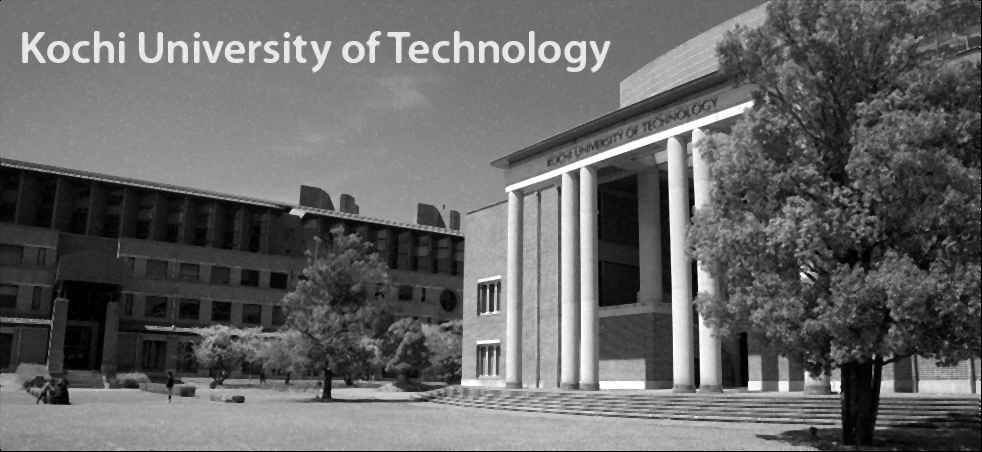
\includegraphics[keepaspectratio,width=\textwidth]{../../Figures/06_24_mf_img_in.png}
            \subcaption{\inimg}
        \end{minipage}
        \caption{メディアンフィルタ適用後の画像}
    \end{minipage}
\end{figure}
\paragraph{Sobelフィルタ,Laplacianフィルタ}
横微分フィルタを適用すると,縦方向のエッジが強調され,縦方向微分フィルタを適用すると,横方向のエッジが強調された.
これらの画像を足し合わせて,\(255\)を上回る値を処理すると,画像全体のエッジが強調された画像を生成できた.
Laplacianフィルタを適用すると,画像が暗く出力された.この画像に対して\figref{fig:Laplacianフィルタのヒストグラム}を用いて,閾値\(30\)の閾値処理し,全体画像のエッジが強調された画像を生成できた.
\begin{figure}[H]
    \centering
    \begin{minipage}[b]{.3\textwidth}
        \centering
        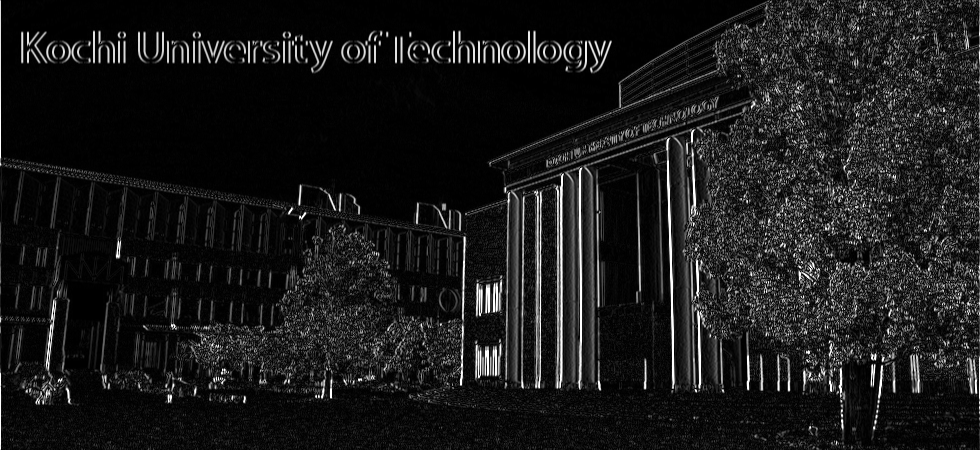
\includegraphics[keepaspectratio,width=\textwidth]{../../Figures/06_31_diff-x-img.png}
        \subcaption{横方向Sobelフィルタ}
    \end{minipage}
    \begin{minipage}[b]{.3\textwidth}
        \centering
        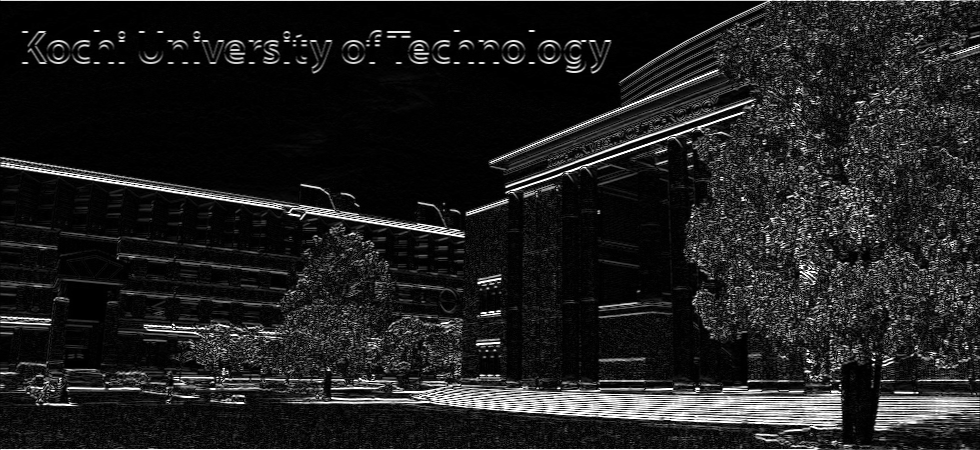
\includegraphics[keepaspectratio,width=\textwidth]{../../Figures/06_32_diff-y-img.png}
        \subcaption{縦方向Sobelフィルタ}
    \end{minipage}
    \begin{minipage}[b]{.3\textwidth}
        \centering
        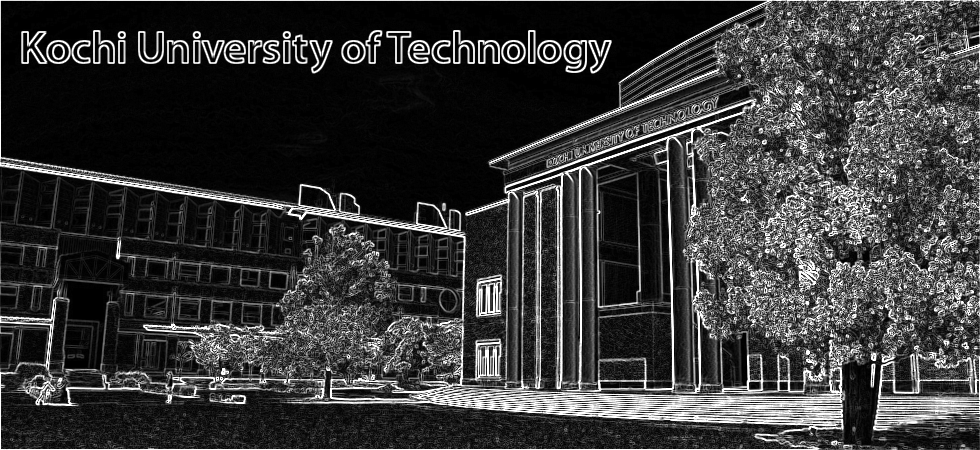
\includegraphics[keepaspectratio,width=\textwidth]{../../Figures/06_33_diff-img.png}
        \subcaption{Sobelフィルタ\footnotemark 適用後の画像}
    \end{minipage}
    \caption{Sobelフィルタの適用}
\end{figure}
\begin{figure}[H]
    \centering
    \begin{minipage}[b]{.3\textwidth}
        \centering
        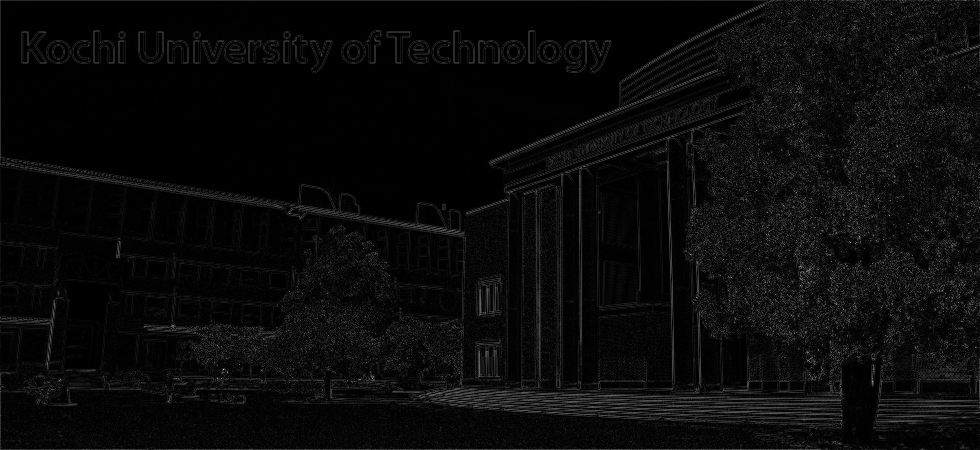
\includegraphics[keepaspectratio,width=\textwidth]{../../Figures/06_41_lf-img}
        \subcaption{Laplacianフィルタ適用後の画像}
    \end{minipage}
    \begin{minipage}[b]{.3\textwidth}
        \centering
        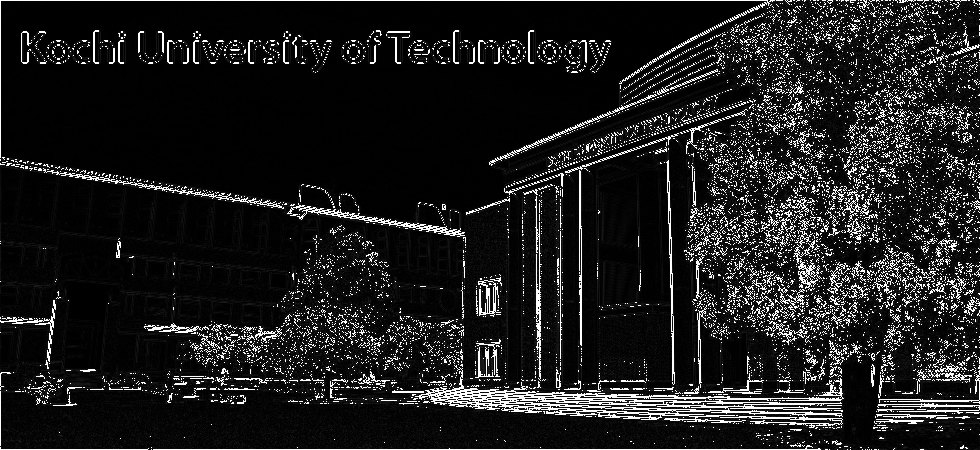
\includegraphics[keepaspectratio,width=\textwidth]{../../Figures/06_43_lf-img-thresholding.png}
        \subcaption{閾値処理\ (閾値\(30\))}
    \end{minipage}
    \begin{minipage}[b]{.3\textwidth}
        \centering
        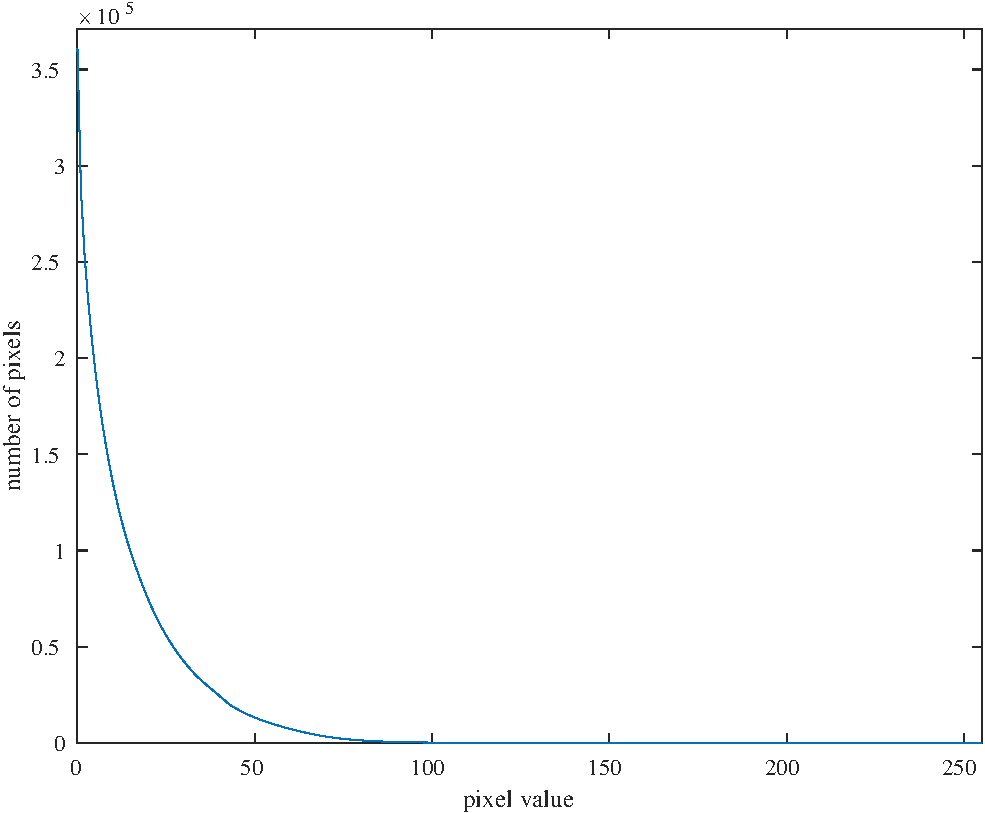
\includegraphics[keepaspectratio,width=\textwidth]{../../Figures/06_42_Thresholding-graph.pdf}
        \subcaption{画素値ヒストグラム}
        \label{fig:Laplacianフィルタのヒストグラム}
    \end{minipage}
    \caption{Laplacianフィルタの適用と処理}
\end{figure}
\footnotetext[1]{横方向Sobelフィルタ適用後画像と縦方向Sobelフィルタ適用後画像の和.}
\begin{figure}[H]
    \centering
    \begin{minipage}[b]{.23\textwidth}
        \centering
        \includegraphics[keepaspectratio,width=\textwidth]{../../06_ImageFiltering/file_hand.png}
        \subcaption{元画像}
    \end{minipage}
    \begin{minipage}[b]{.23\textwidth}
        \centering
        \includegraphics[keepaspectratio,width=\textwidth]{../../Figures/06_51_img-hsv.png}
        \subcaption{HSV色空間への変換後}
    \end{minipage}
    \begin{minipage}[b]{.23\textwidth}
        \centering
        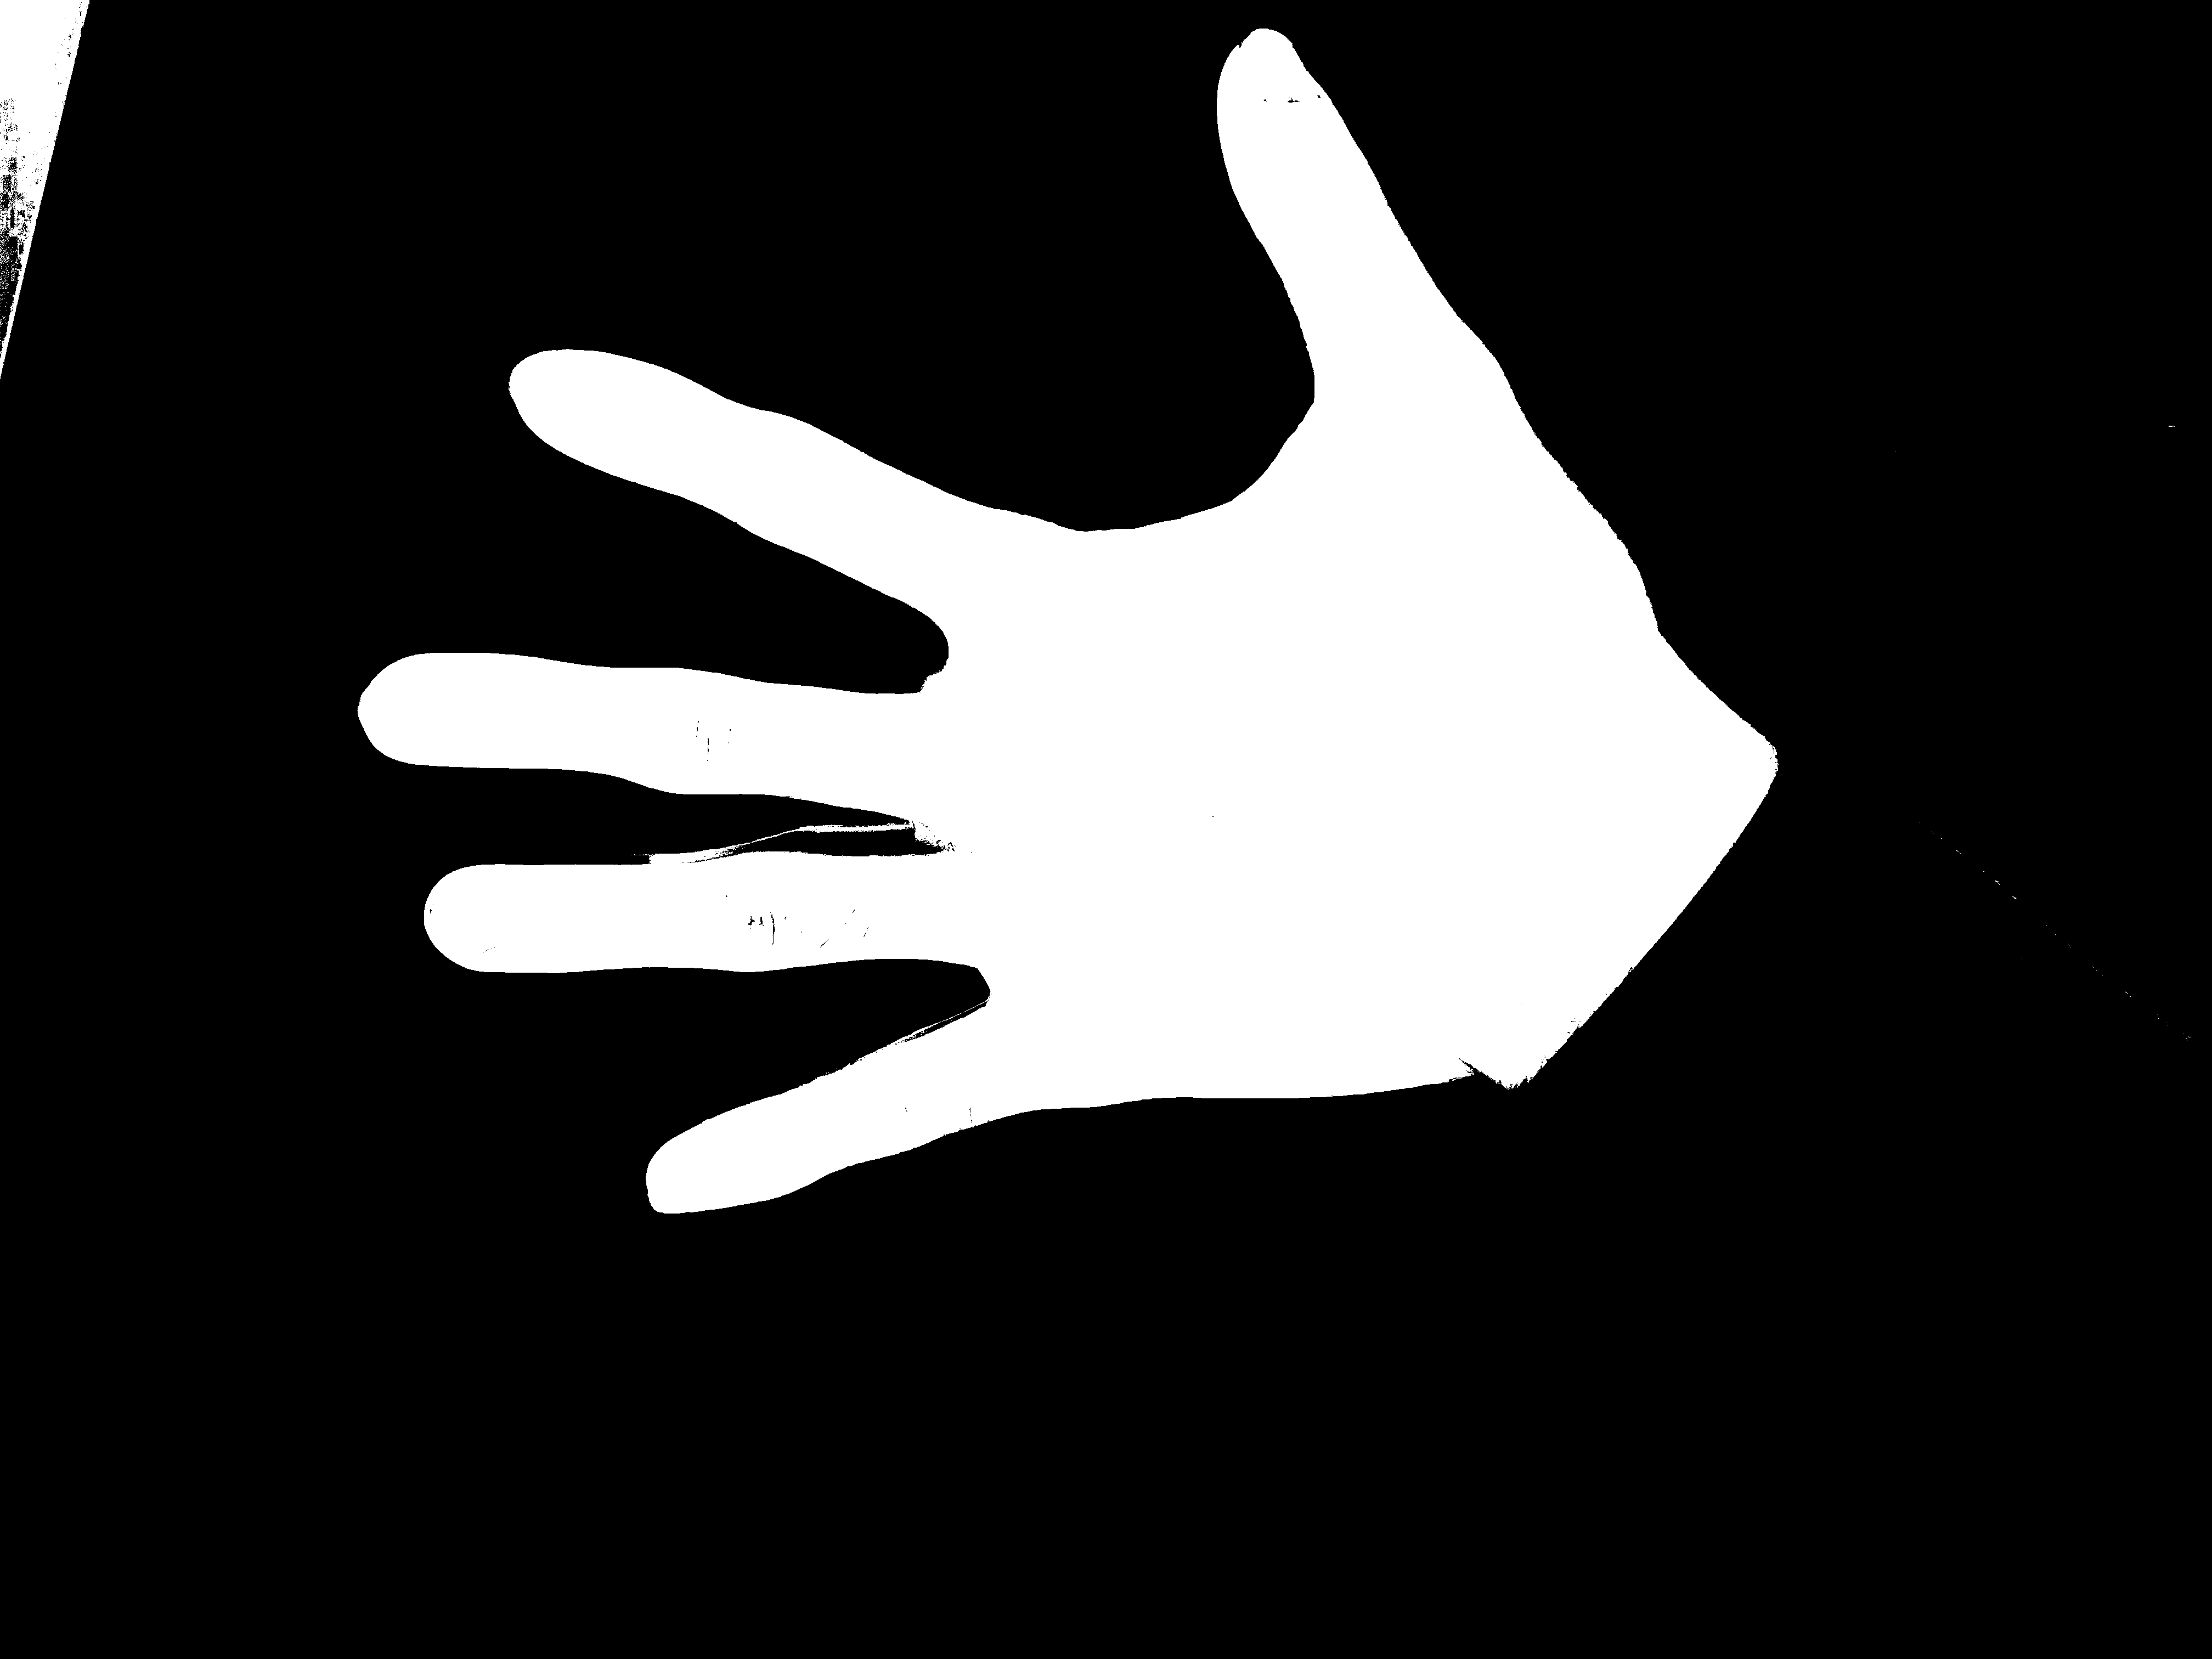
\includegraphics[keepaspectratio,width=\textwidth]{../../Figures/06_52_scd.png}
        \subcaption{肌色領域の抽出(HSV)}
    \end{minipage}
    \begin{minipage}[b]{.23\textwidth}
        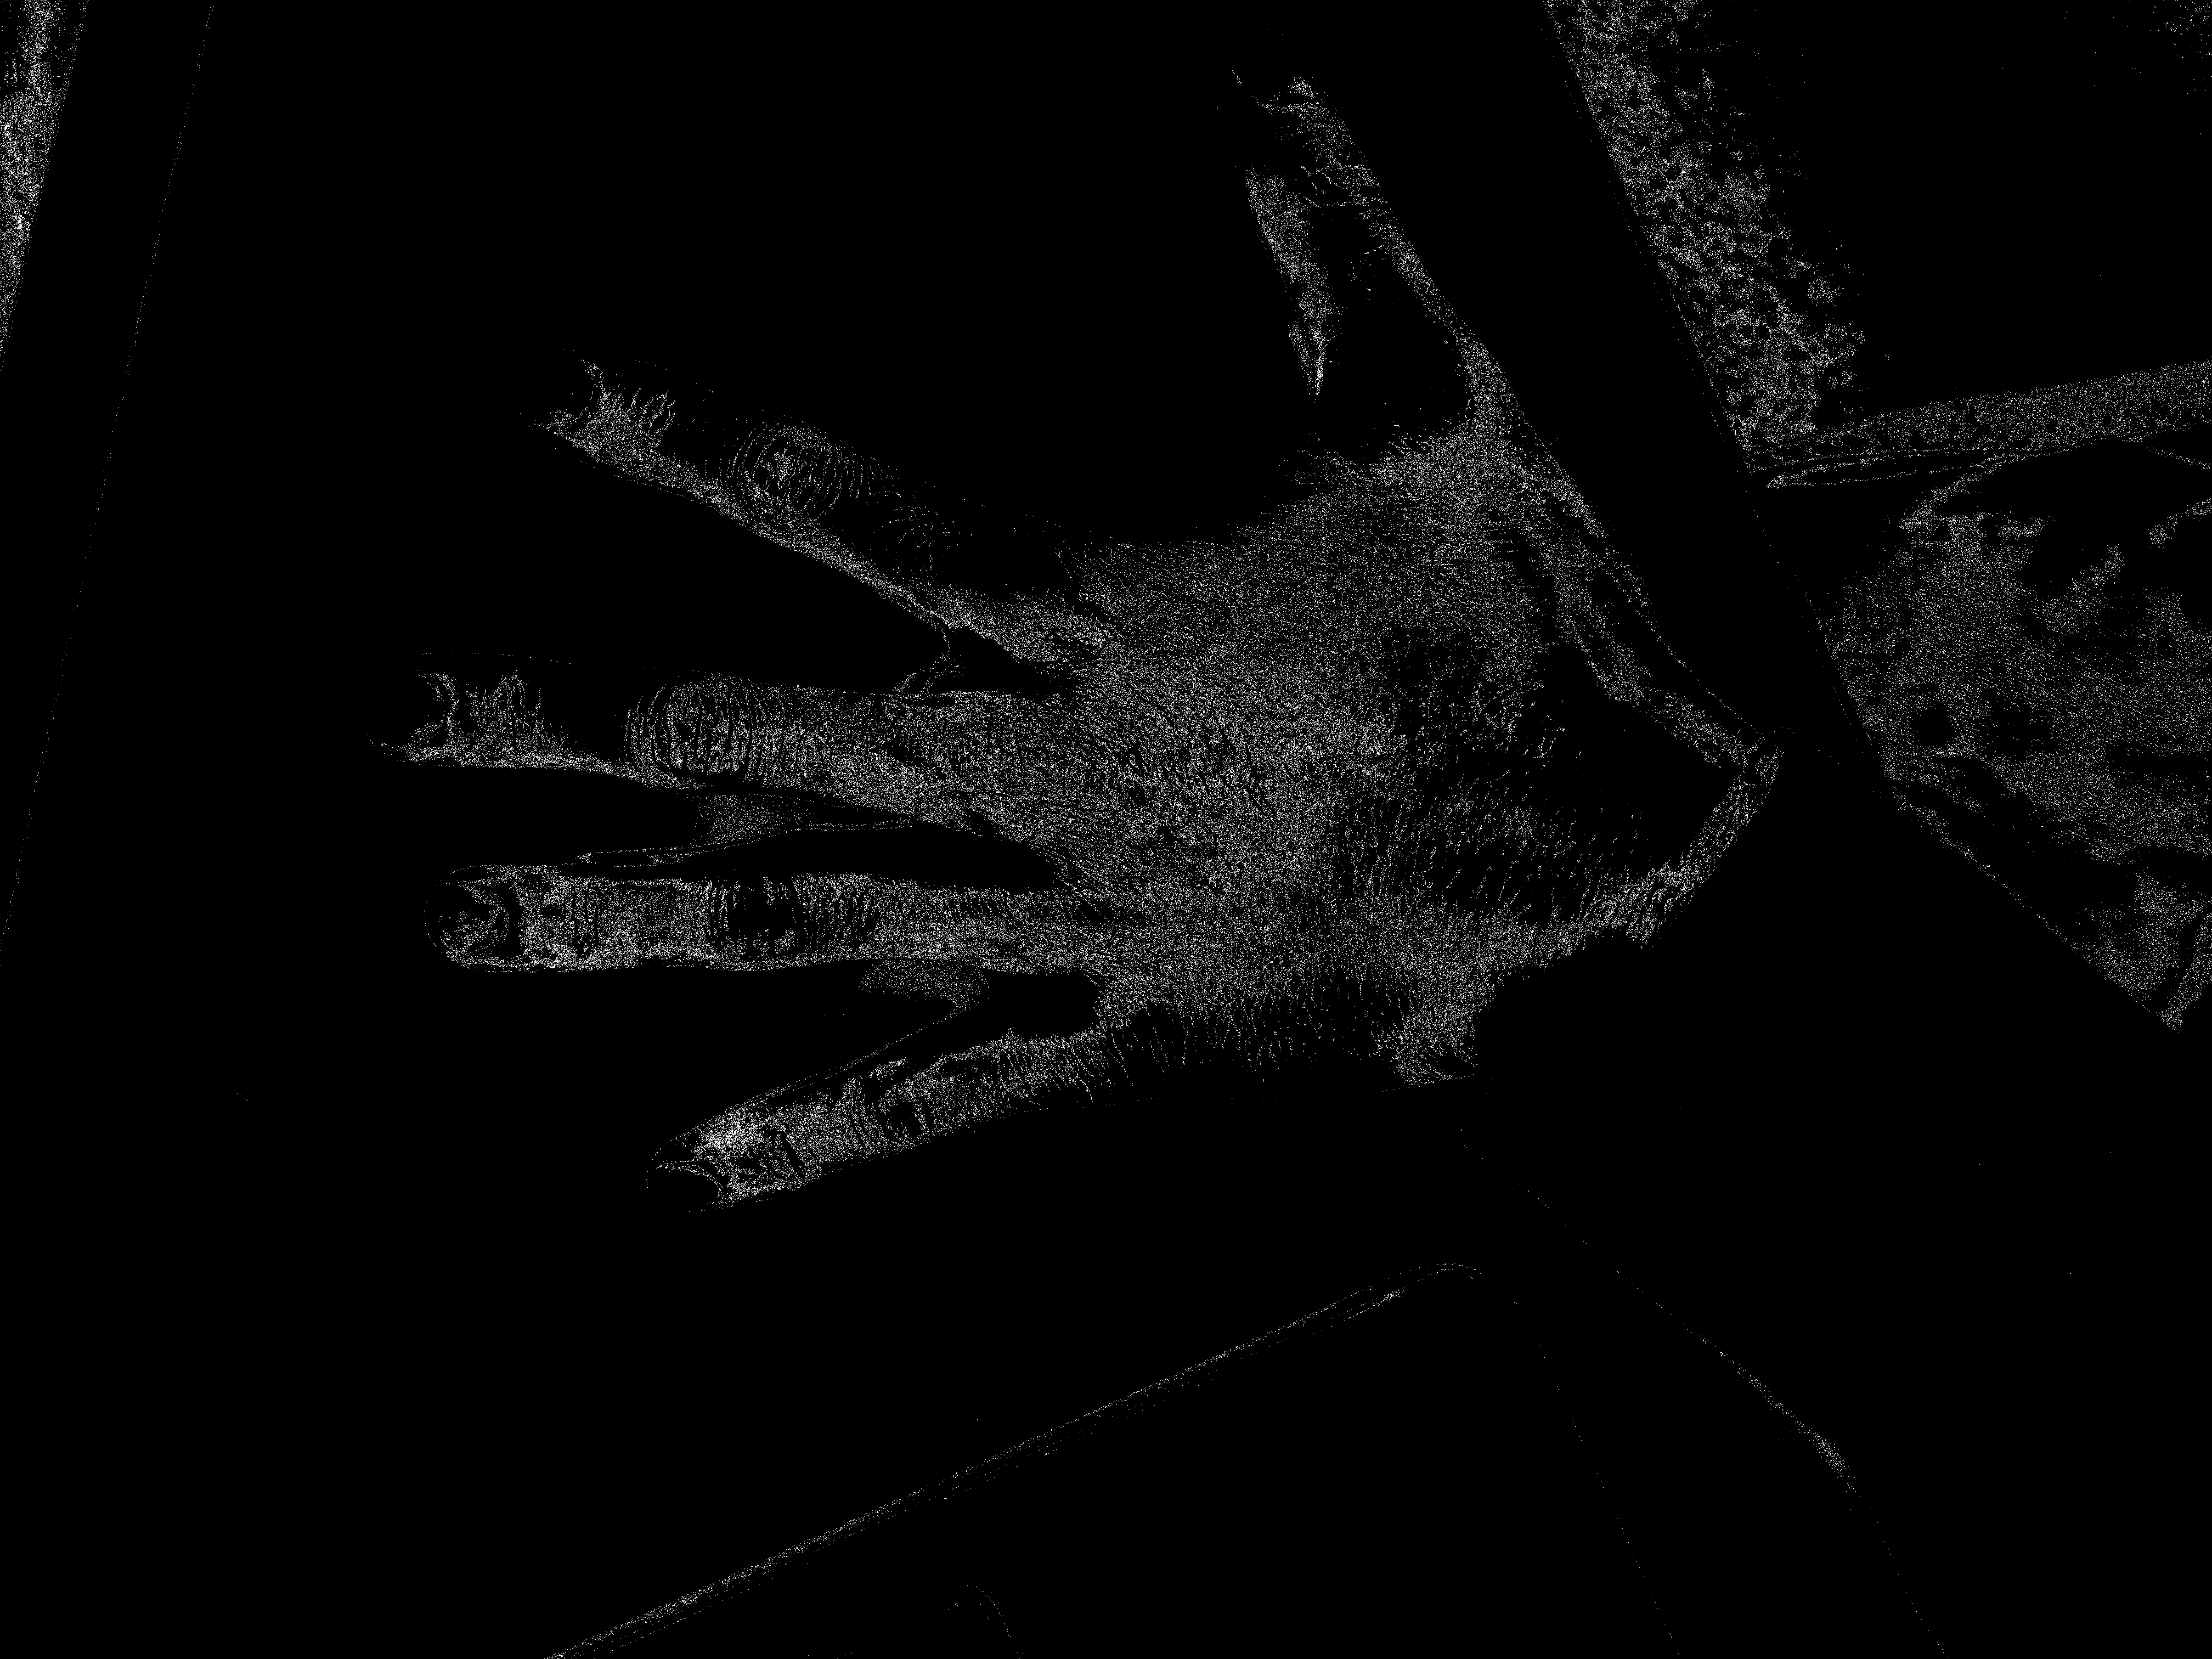
\includegraphics[keepaspectratio,width=\textwidth]{../../Figures/06_53_hand.png}
        \subcaption{肌色領域の抽出(RGB)}
    \end{minipage}
    \caption{\kadaibe\ 実験結果}
\end{figure}
\newpage
\begin{figure}[H]
    \centering
    \renewcommand{\arraystretch}{1.5}
    \begin{tabularx}{\textwidth}{p{.05\textwidth}CCC}
                                                                                                & {\small 縞数\(4\)} & {\small 縞数\(16\)} & {\small 縞数\(64\)} \\
        \begin{minipage}{.05\textwidth}
            \centering
            \rotatebox{90}{縦縞}
        \end{minipage}                                                         &
        \begin{minipage}{.25\textwidth}
            \centering
            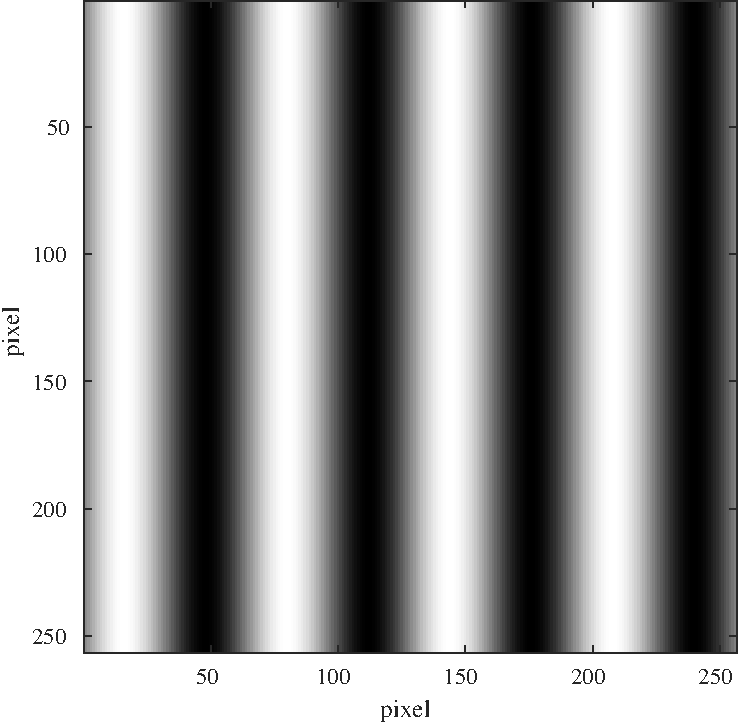
\includegraphics[width=.9\textwidth,keepaspectratio]{../../Figures/08_11_img4.pdf}
        \end{minipage}      &
        \begin{minipage}{.25\textwidth}
            \centering
            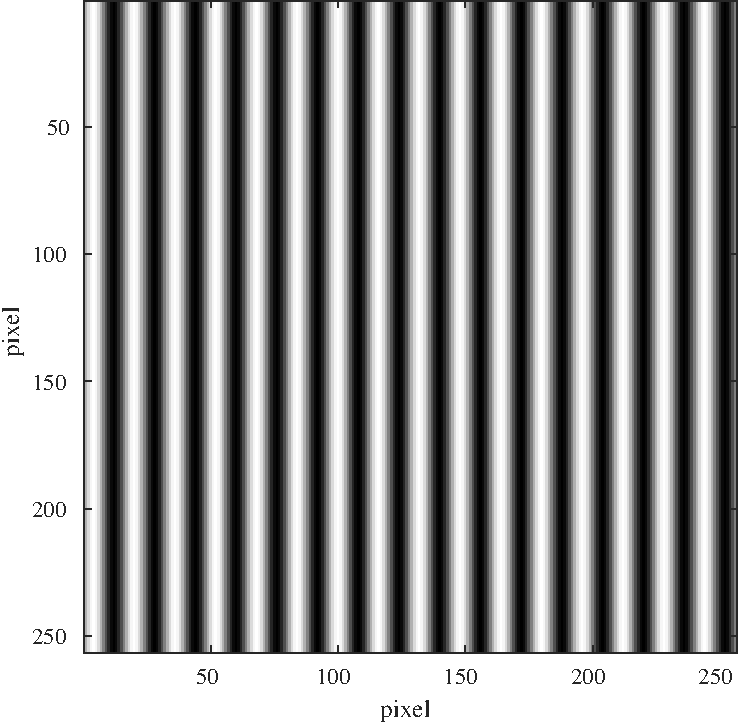
\includegraphics[width=.9\textwidth,keepaspectratio]{../../Figures/08_12_img16.pdf}
        \end{minipage}     &
        \begin{minipage}{.25\textwidth}
            \centering
            
\includegraphics[width=.9\textwidth,keepaspectratio]{../../Figures/08_13_img64.pdf}
        \end{minipage}                                                                 \\

        \begin{minipage}{.05\textwidth}
            \centering
            \rotatebox{90}{\small 縦縞\ パワースペクトル}
        \end{minipage}                                                     &
        \begin{minipage}{.25\textwidth}
            \centering
            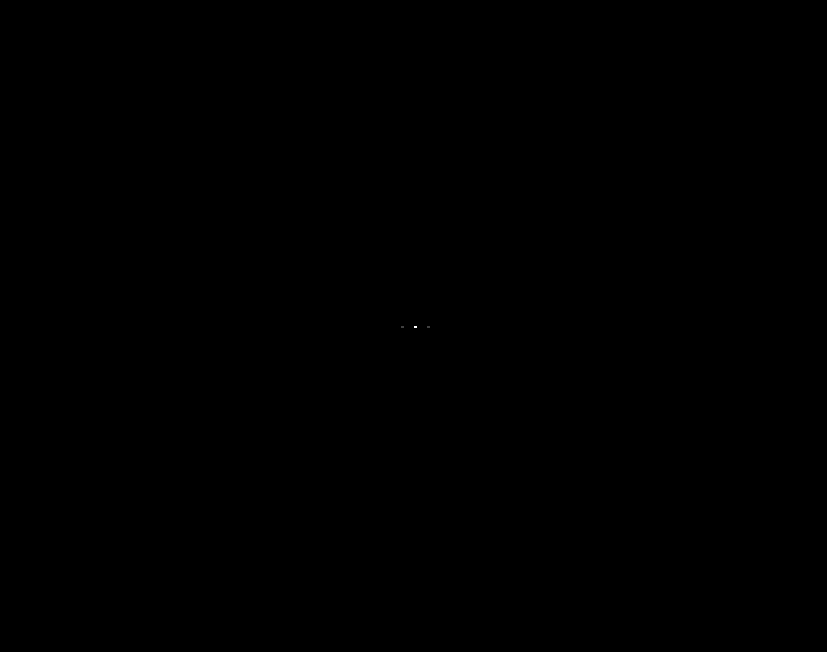
\includegraphics[keepaspectratio,width=.9\textwidth]{../../Figures/08_14_img4-fft.pdf}
        \end{minipage}  &
        \begin{minipage}{.25\textwidth}
            \centering
            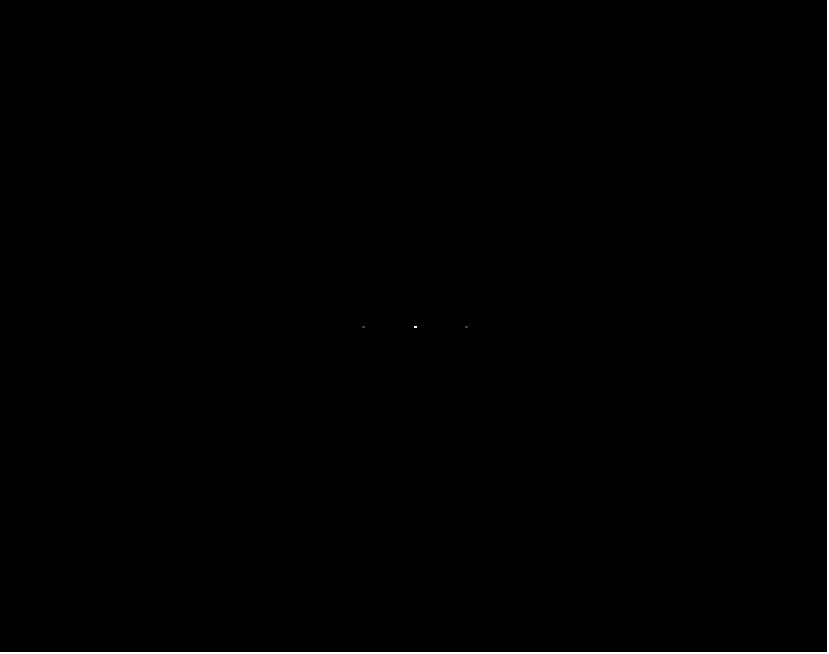
\includegraphics[keepaspectratio,width=.9\textwidth]{../../Figures/08_15_img16-fft.pdf}
        \end{minipage} &
        \begin{minipage}{.25\textwidth}
            \centering
            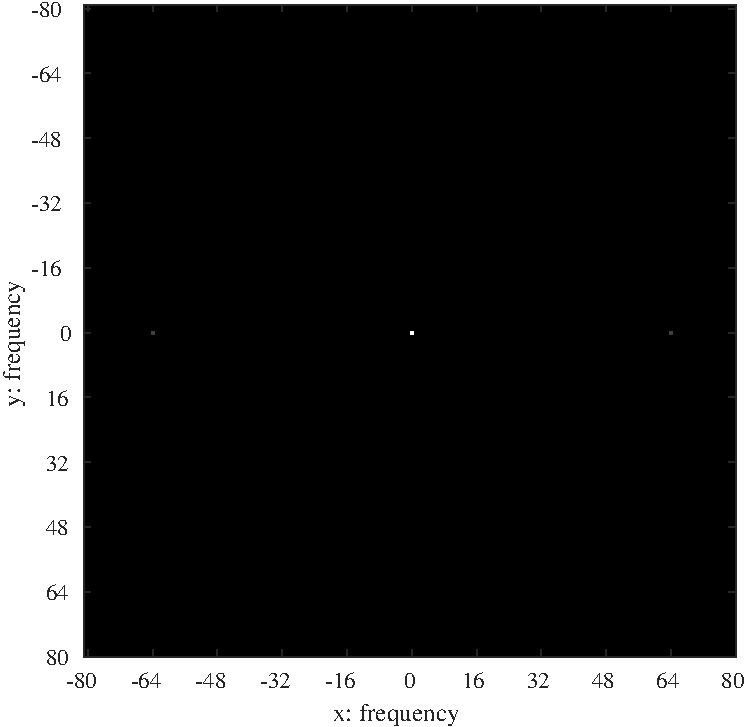
\includegraphics[keepaspectratio,width=.9\textwidth]{../../Figures/08_16_img64-fft.pdf}
        \end{minipage}                                                             \\

        \begin{minipage}{.05\textwidth}
            \centering
            \rotatebox{90}{横縞}
        \end{minipage}                                                         &
        \begin{minipage}{.25\textwidth}
            \centering
            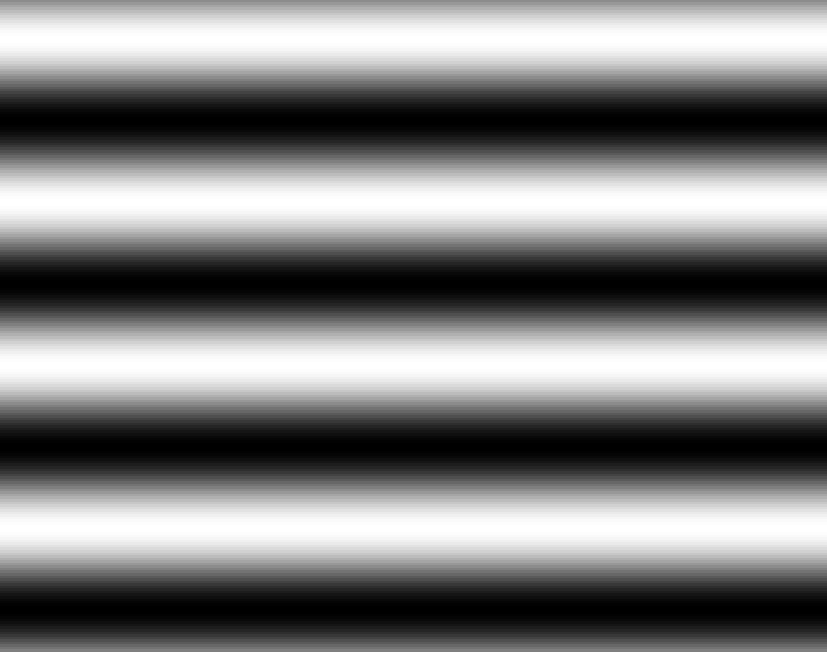
\includegraphics[width=.9\textwidth,keepaspectratio]{../../Figures/08_21_img4.pdf}
        \end{minipage}      &
        \begin{minipage}{.25\textwidth}
            \centering
            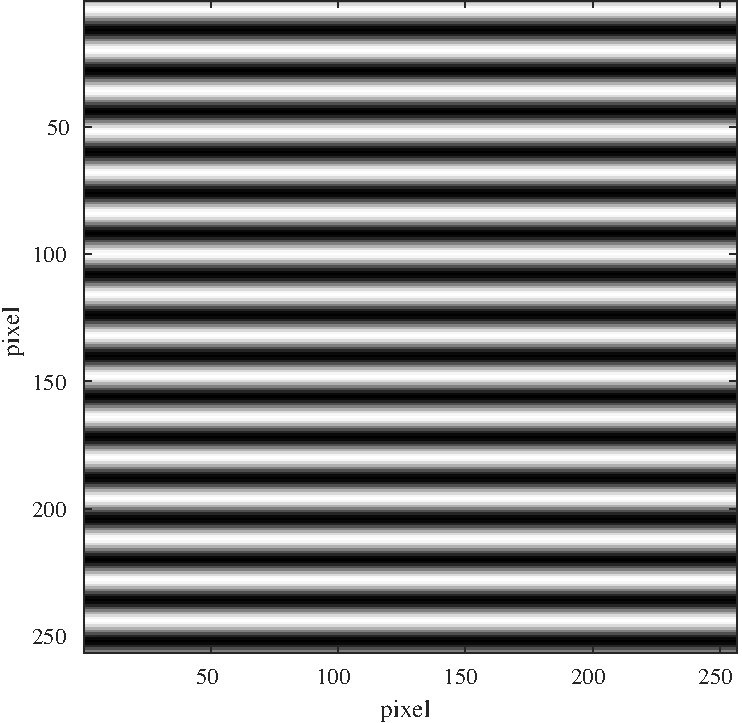
\includegraphics[width=.9\textwidth,keepaspectratio]{../../Figures/08_22_img16.pdf}
        \end{minipage}     &
        \begin{minipage}{.25\textwidth}
            \centering
            
\includegraphics[width=.9\textwidth,keepaspectratio]{../../Figures/08_23_img64.pdf}
        \end{minipage}                                                                 \\

        \begin{minipage}{.05\textwidth}
            \centering
            \rotatebox{90}{\small 横縞\ パワースペクトル}
        \end{minipage}                                                     &
        \begin{minipage}{.25\textwidth}
            \centering
            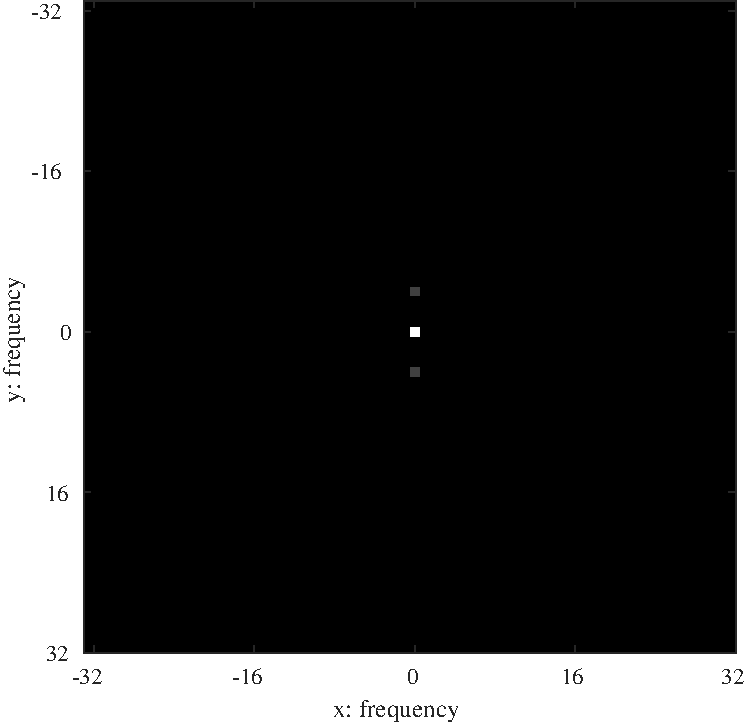
\includegraphics[keepaspectratio,width=.9\textwidth]{../../Figures/08_24_img4-fft.pdf}
        \end{minipage}  &
        \begin{minipage}{.25\textwidth}
            \centering
            \includegraphics[keepaspectratio,width=.9\textwidth]{../../Figures/08_25_img16-fft.pdf}
        \end{minipage} &
        \begin{minipage}{.25\textwidth}
            \centering
            \includegraphics[keepaspectratio,width=.9\textwidth]{../../Figures/08_26_img64-fft.pdf}
        \end{minipage}                                                             \\
    \end{tabularx}
    \caption{縦縞・横縞に対するフーリエ変換}
\end{figure}
\paragraph{2次元フーリエ変換}
長方形の座標による,対数をとったパワースペクトルの違いは,目視で確認できなかった.ただし,両パワースペクトルの差分を取った行列の最大値,最小値を調べると,いずれも\(0\)ではなかった.
\begin{figure}[H]
    \centering
    \begin{minipage}[b]{.2\textwidth}
        \centering
        \includegraphics[keepaspectratio,width=\textwidth]{../../Figures/08_31_rec1.pdf}
        \subcaption{長方形\ 1}
    \end{minipage}
    \begin{minipage}[b]{.2\textwidth}
        \centering
        \includegraphics[keepaspectratio,width=\textwidth]{../../Figures/08_32_rec2.pdf}
        \subcaption{長方形\ 2}
    \end{minipage}
    \begin{minipage}[b]{.25\textwidth}
        \centering
        \includegraphics[keepaspectratio,width=.8\textwidth]{../../Figures/08_33_rec1-fft.pdf}
        \subcaption{長方形\ 1\ パワースペクトル}
    \end{minipage}
    \begin{minipage}[b]{.25\textwidth}
        \centering
        \includegraphics[keepaspectratio,width=.8\textwidth]{../../Figures/08_34_rec2-fft.pdf}
        \subcaption{長方形\ 2\ パワースペクトル}
    \end{minipage}
    \caption{画像の座標とパワースペクトルの関係}
\end{figure}
\begin{figure}[H]
    \centering
    \begin{minipage}[b]{.23\textwidth}
        \centering
        \includegraphics[keepaspectratio,width=\textwidth]{../../LENNA.jpeg}
        \subcaption{元画像}
    \end{minipage}
    \begin{minipage}[b]{.23\textwidth}
        \centering
        \includegraphics[keepaspectratio,width=\textwidth]{../../Figures/08_41_filter.pdf}
        \subcaption{円形フィルタ\footnotemark[1]}
    \end{minipage}
    \begin{minipage}[b]{.23\textwidth}
        \centering
        \includegraphics[keepaspectratio,width=\textwidth]{../../Figures/08_42_fft.pdf}
        \subcaption{パワースペクトル}
    \end{minipage}
    \begin{minipage}[b]{.23\textwidth}
        \centering
        \includegraphics[keepaspectratio,width=\textwidth]{../../Figures/08_43_fft-filter.pdf}
        \subcaption{フィルタの適用\footnotemark[1]}
    \end{minipage}
    \begin{minipage}[b]{.48\textwidth}
        \centering
        \includegraphics[keepaspectratio,width=\textwidth]{../../Figures/08_44_fft-filter-50.pdf}
        \subcaption{フィルタ適用後\((50)\)}
    \end{minipage}
    \begin{minipage}[b]{.48\textwidth}
        \centering
        \includegraphics[keepaspectratio,width=\textwidth]{../../Figures/08_45_fft-filter-100.pdf}
        \subcaption{フィルタ適用後\((100)\)}
    \end{minipage}
    \caption{高域通過フィルタ}
\end{figure}
\footnotetext[1]{例として,半径が\(50\textrm{pixel}\)のフィルタを示す.}